%%%%%%%%%%%%%%%%%%%%%%%%%%%%%%%%%%%%%%%%%
% Journal Article
% LaTeX Template
% Version 1.4 (15/5/16)
%
% This template has been downloaded from:
% http://www.LaTeXTemplates.com
%
% Original author:
% Frits Wenneker (http://www.howtotex.com) with extensive modifications by
% Vel (vel@LaTeXTemplates.com)
%
% License:
% CC BY-NC-SA 3.0 (http://creativecommons.org/licenses/by-nc-sa/3.0/)
%
%%%%%%%%%%%%%%%%%%%%%%%%%%%%%%%%%%%%%%%%%

%----------------------------------------------------------------------------------------
%	PACKAGES AND OTHER DOCUMENT CONFIGURATIONS
%----------------------------------------------------------------------------------------

\documentclass{article}

\usepackage{blindtext} % Package to generate dummy text throughout this template 

\usepackage[sc]{mathpazo} % Use the Palatino font
\usepackage[T1]{fontenc} % Use 8-bit encoding that has 256 glyphs
\linespread{1.25} % Line spacing - Palatino needs more space between lines
\usepackage{microtype} % Slightly tweak font spacing for aesthetics

\usepackage[english]{babel} % Language hyphenation and typographical rules

\usepackage[hmarginratio=1:1,top=32mm,columnsep=20pt]{geometry} % Document margins
\usepackage[hang, small,labelfont=bf,up,textfont=it,up]{caption} % Custom captions under/above floats in tables or figures
\usepackage{booktabs} % Horizontal rules in tables

\usepackage{lettrine} % The lettrine is the first enlarged letter at the beginning of the text

\usepackage{enumitem} % Customized lists
\setlist[itemize]{noitemsep} % Make itemize lists more compact

\usepackage{abstract} % Allows abstract customization
\renewcommand{\abstractnamefont}{\normalfont\bfseries} % Set the "Abstract" text to bold
\renewcommand{\abstracttextfont}{\normalfont\small\itshape} % Set the abstract itself to small italic text

\usepackage{titlesec} % Allows customization of titles
\renewcommand\thesection{\Roman{section}} % Roman numerals for the sections
\renewcommand\thesubsection{\roman{subsection}} % roman numerals for subsections
\titleformat{\section}[block]{\large\scshape\centering}{\thesection.}{1em}{} % Change the look of the section titles
\titleformat{\subsection}[block]{\large}{\thesubsection.}{1em}{} % Change the look of the section titles

\usepackage{fancyhdr} % Headers and footers
\pagestyle{fancy} % All pages have headers and footers
\fancyhead{} % Blank out the default header
\fancyfoot{} % Blank out the default footer
% \fancyhead[C]{Running title $\bullet$ May 2016 $\bullet$ Vol. XXI, No. 1} % Custom header text
\fancyfoot[RO,LE]{\thepage} % Custom footer text

\usepackage{titling} % Customizing the title section

\usepackage[hidelinks]{hyperref} % For hyperlinks in the PDF
\usepackage{graphicx}
\graphicspath{{figures/}}

\usepackage{subfig}

\usepackage{booktabs}

%--------------------------------

%Import the natbib package and sets a bibliography  and citation styles
\usepackage{natbib}
\bibliographystyle{abbrvnat}
\setcitestyle{authoryear,open={(},close={)}}

% \usepackage[
%     backend=biber,
%     style=authoryear,
%     citestyle=unsrt,
% ]{biblatex}
% \usepackage{csquotes}

% \addbibresource{sample.bib}
%--------------------------------

%----------------------------------------------------------------------------------------
%	TITLE SECTION
%----------------------------------------------------------------------------------------

\setlength{\droptitle}{-4\baselineskip} % Move the title up

\pretitle{\begin{center}\Huge\bfseries} % Article title formatting
\posttitle{\end{center}} % Article title closing formatting
\title{Detecting Linguistic Change in Reddit's \textit{The\_Donald}} % Article title
\author{%
% \textsc{John Smith}\thanks{A thank you or further information} \\[1ex] % Your name
\textsc{Adarsh Mathew} \\[1ex] % Your name
\normalsize Final Paper, Computational Content Analysis (Winter 2020) \\ % Your institution
\normalsize \href{mailto:adarshm@uchicago.edu}{adarshm@uchicago.edu} % Your email address
%\and % Uncomment if 2 authors are required, duplicate these 4 lines if more
%\textsc{Jane Smith}\thanks{Corresponding author} \\[1ex] % Second author's name
%\normalsize University of Utah \\ % Second author's institution
%\normalsize \href{mailto:jane@smith.com}{jane@smith.com} % Second author's email address
}

% \date{\today} % Leave empty to omit a date
\date{} % Leave empty to omit a date

\renewcommand{\maketitlehookd}{%

% \begin{abstract}
% \noindent \blindtext % Dummy abstract text - replace \blindtext with your abstract text
% \end{abstract}

}

%----------------------------------------------------------------------------------------

\begin{document}

% Print the title
\maketitle

%----------------------------------------------------------------------------------------
%	ARTICLE CONTENTS
%----------------------------------------------------------------------------------------

\section{Background}

% \lettrine[nindent=0em,lines=3]{L}  

As the world increasingly comes online, one should expect a version of our political activities being performed on these platforms too. The affordances of the internet and networked platforms like Twitter, Reddit, and Facebook reduce the transaction costs of engagement at scale. By reducing the cost of content creation and downgrading the importance of traditional mediators of attention and political influence like the news media, platforms have enabled the amplification and shaping of erstwhile niche or marginalized narratives. These very affordances make political communication and activism a natural fit for actors on these platforms.

Political communication has always relied on tapping into pop culture to make its message more palatable to the public and likely voters. This has extended to digital politics too: political memes perform the role of satire, candidates maintain a presence across multiple platforms, which pollsters and campaigns rely on for fundraising and electoral analysis. But digital politics also means that a candidate or party's messaging on these platforms cannot be a controlled and mediated spectacle like it could have been in traditional media. Near-instant feedback and engagement, algorithmic amplification, and the sheer scale of platforms create an ecosystem where no campaign can reasonably hope to exert top-down control on narratives, messaging, and language. 

If President Obama's re-relection in 2012 was the first US presidential election that relied on social media for targeted messaging, Donald Trump's election win in 2016 marked the next stage of digital politics, driven by micro-targeted advertising, candidate tweets, data breaches, and disinformation campaigns. In addition to their messaging success, Trump's base proved to be extremely good at setting the agenda -- re-framing the controversy around Hillary Clinton's e-mails as a referendum on her lack of honesty, the overtly racist framing on issues like `Black Lives Matter', etc. Users of 4chan/8chan's r/pol/and reddit's \textit{r/The\_Donald} were able to command attention online, driving their narrative through memes and highly specific language familiar to digital natives. In light of all this, how does one track the changing context around issues in these communities? How does a user's linguistic behaviour change with greater engagement? How does one measure the embedded context around political entities on these forums?   

President Donald Trump’s rise has been associated with the rise to prominence of far-right communities, branded as the ‘alt-right’. The violent, ostensibly supremacist ‘Unite the Right’ rally in Charlottesville, Virginia was seen by many as a watershed moment that marked the rise of this subgroup \citep{atkinson_charlottesville_2018}. President Trump’s election campaign itself was marked by several racist and misogynistic statements, which were cheered on wildly and amplified by this subgroup. Heikkilä argues that by actively antagonizing both Democrats and classic conservatives -- through memes and online culture wars -- the alt-right pushed the conversation farther to the right, normalized the vilification of ‘political correctness’, and created a feedback loop that rewarded the campaign for its extreme positions \citep{heikkila_online_2017, nagle_kill_2017}. 

The tactics of the alt-right are heavily influenced by the 'ironic' meme culture of 4chan/8chan. The origins and inspirations for its more virulent side, which includes shitposting, bullying, targeted harrassment, doxxing (release of private information), can be traced to 'GamerGate'. ‘GamerGate’ refers to the targeted harassment of video game journalists  orchestrated through the hashtag '\#GamerGate'. Beginning in August 2014, it involved the large-scale coordinated harassment of specific women video game journalists who were critical of the portrayal of women in video games. Characterized as an effort to resist the imposition of politically correct norms on the art they love, the community lashed out at specific targets. Victims received death threats, rape threats, their addresses were posted online (doxxing). GamerGate was a vital moment in the crystallization of the alt-right as we know it \citep{blodgett_ghostbusters_2018}. The alt-right embraced the tactics of GamerGate, employing and co-opting the meme-first approach to discourse, along with a full-throated disavowal of feminist, politically-correct discourse. All of this was interspersed with 'ironic' jokes replete with racist, anti-Semitic, and misogynistic themes.

The importance of GamerGate in understanding the alt-right movement cannot be understated -- the incident tapped into a well of discontent in a population that wielded a lot of power in the online world, but felt marginalized. The misogynistic nature of the alt-right's fundamental beliefs have been touched upon by academics and journalists. The alt-right is defined by its white supremacist and anti-Semitic ideology, but when alt-right members talk about the women who are standing between them and their “rightful” position, their language is virtually indistinguishable from what you can find on misogynistic message boards \citep{league2018women}. The subculture is characterized by its extreme disavowal of 'political correctness' and its norms, along with the 'Social Justice Warriors' who enforce it online. They're strongly opposed to Feminist values; 'Feminism is Cancer' continues to be one of the most popular memes of the alt-right, and still serves as a rallying cry. Casting themselves as noble warriors defending the sanctity of what they love, young, white men -- railing against the enforced ‘politically correct’ critiques of the video-game industry -- engaged in coordinated, large-scale, targeted harassment while being cheered on gleefully \citep{nieborg_mainstreaming_2018}. The actions of key players set the norms for the community, and normalized a vicious version of internet ‘trolling’, giving birth to a plethora of celebrities like Milo Yiannopoulous, who modelled himself as an ‘anti-feminist, ultra-conservative bad boy’ \citep{koulouris_online_2018}. It provided a blueprint for reactionary mobilization and engagement on the internet \citep{daniels_algorithmic_2018}. 
  
In this paper, I attempt to understand how linguistic behaviour of users in online communities have changed over time, and what the relationship between the language of prominent users and the community at large looks like. I also seek to quantify how the context around key phrases has changed over time using word embedding methods. Additionally, using word embeddings, I construct dimensions of key electoral issues and track how the perception of political figures and institutions shift on these dimensions. 

%------------------------------------------------

\section{Methods}

\subsection*{Data Sources}

I use data from the \textit{r/The\_Donald} subreddit to track and understand changes in user linguistic and rhetoric behaviour over time. Using a combination of the Reddit API\footnote{Reddit API: https://www.reddit.com/dev/api/} and the pushshift.io API\footnote{Pushshift API: https://pushshift.io/api-parameters/} \citep{baumgartner_pushshift_2020}, I use all submissions and comments made from 16 June 2015 to 8 November 2018 as my corpus of text. This totals almost 2.3 million unique entries for a period of 40 months. The data collection tracks the subreddit from when President Trump announced his candidacy to the two-year anniversary of his election win. 

\subsection*{Snapshot Language Models \& User Change}

To quantify changes in user lingusitic behaviour relative to the community, I adapt the methodology used by Danescu-Niculescu-Mizil et al.'s 2013 paper \textit{No Country for Old Members} \citep{danescu-niculescu-mizil_no_2013}. I use a bi-gram Snapshot Language Model ($SLM$) with normalized tokens. I use the Interpolated Kneser-Ney smoothing method, which mixes a discounted probability with a lower-order continuation probability, with a discount factor of $d = 0.1$\footnote{The default discount factor in Python's \texttt{nltk} library is set to 0.1.}. Kneser-Ney smoothing makes use of the probability of a word being a novel continuation. While Danescu-Niculescu-Mizil et al use a Katz back-off smoothing approach tuned on a held-out set, I choose Kneser-Ney Interpolation for its superior performance \citep{jurafsky_speech_2008}. The duration of each snapshot is 6 weeks, thus generating $30$ such windows to examine user and sub-group behaviour.

For each post in a six-week window, I compute its cross-entropy according to the $SLM_{w(p)}$ of the window. This cross-entropy is a measure of how surprising the language of the post is relative to the language of the subreddit in the window. Higher cross-entropy values indicate greater deviation from the language of the subreddit.  Like Danescu-Niculescu-Mizil et al., I only consider the first 5 sentences of each post to calculate the cross-entropy metric; longer posts would have higher cross-entropy, so a hard limit of $k = 5$ makes it possible to compare cross-entropy scores across posts. Due to considerations of computation time, I only examine submissions and not comments for this method. Additionally, I calculate cross-entropy for posts which have 10 comments or more, have a score of 100 or more. I drop the first 5 and last period, giving us almost 230k posts over 23 periods to examine.

\begin{figure}[t]%

    \centering

    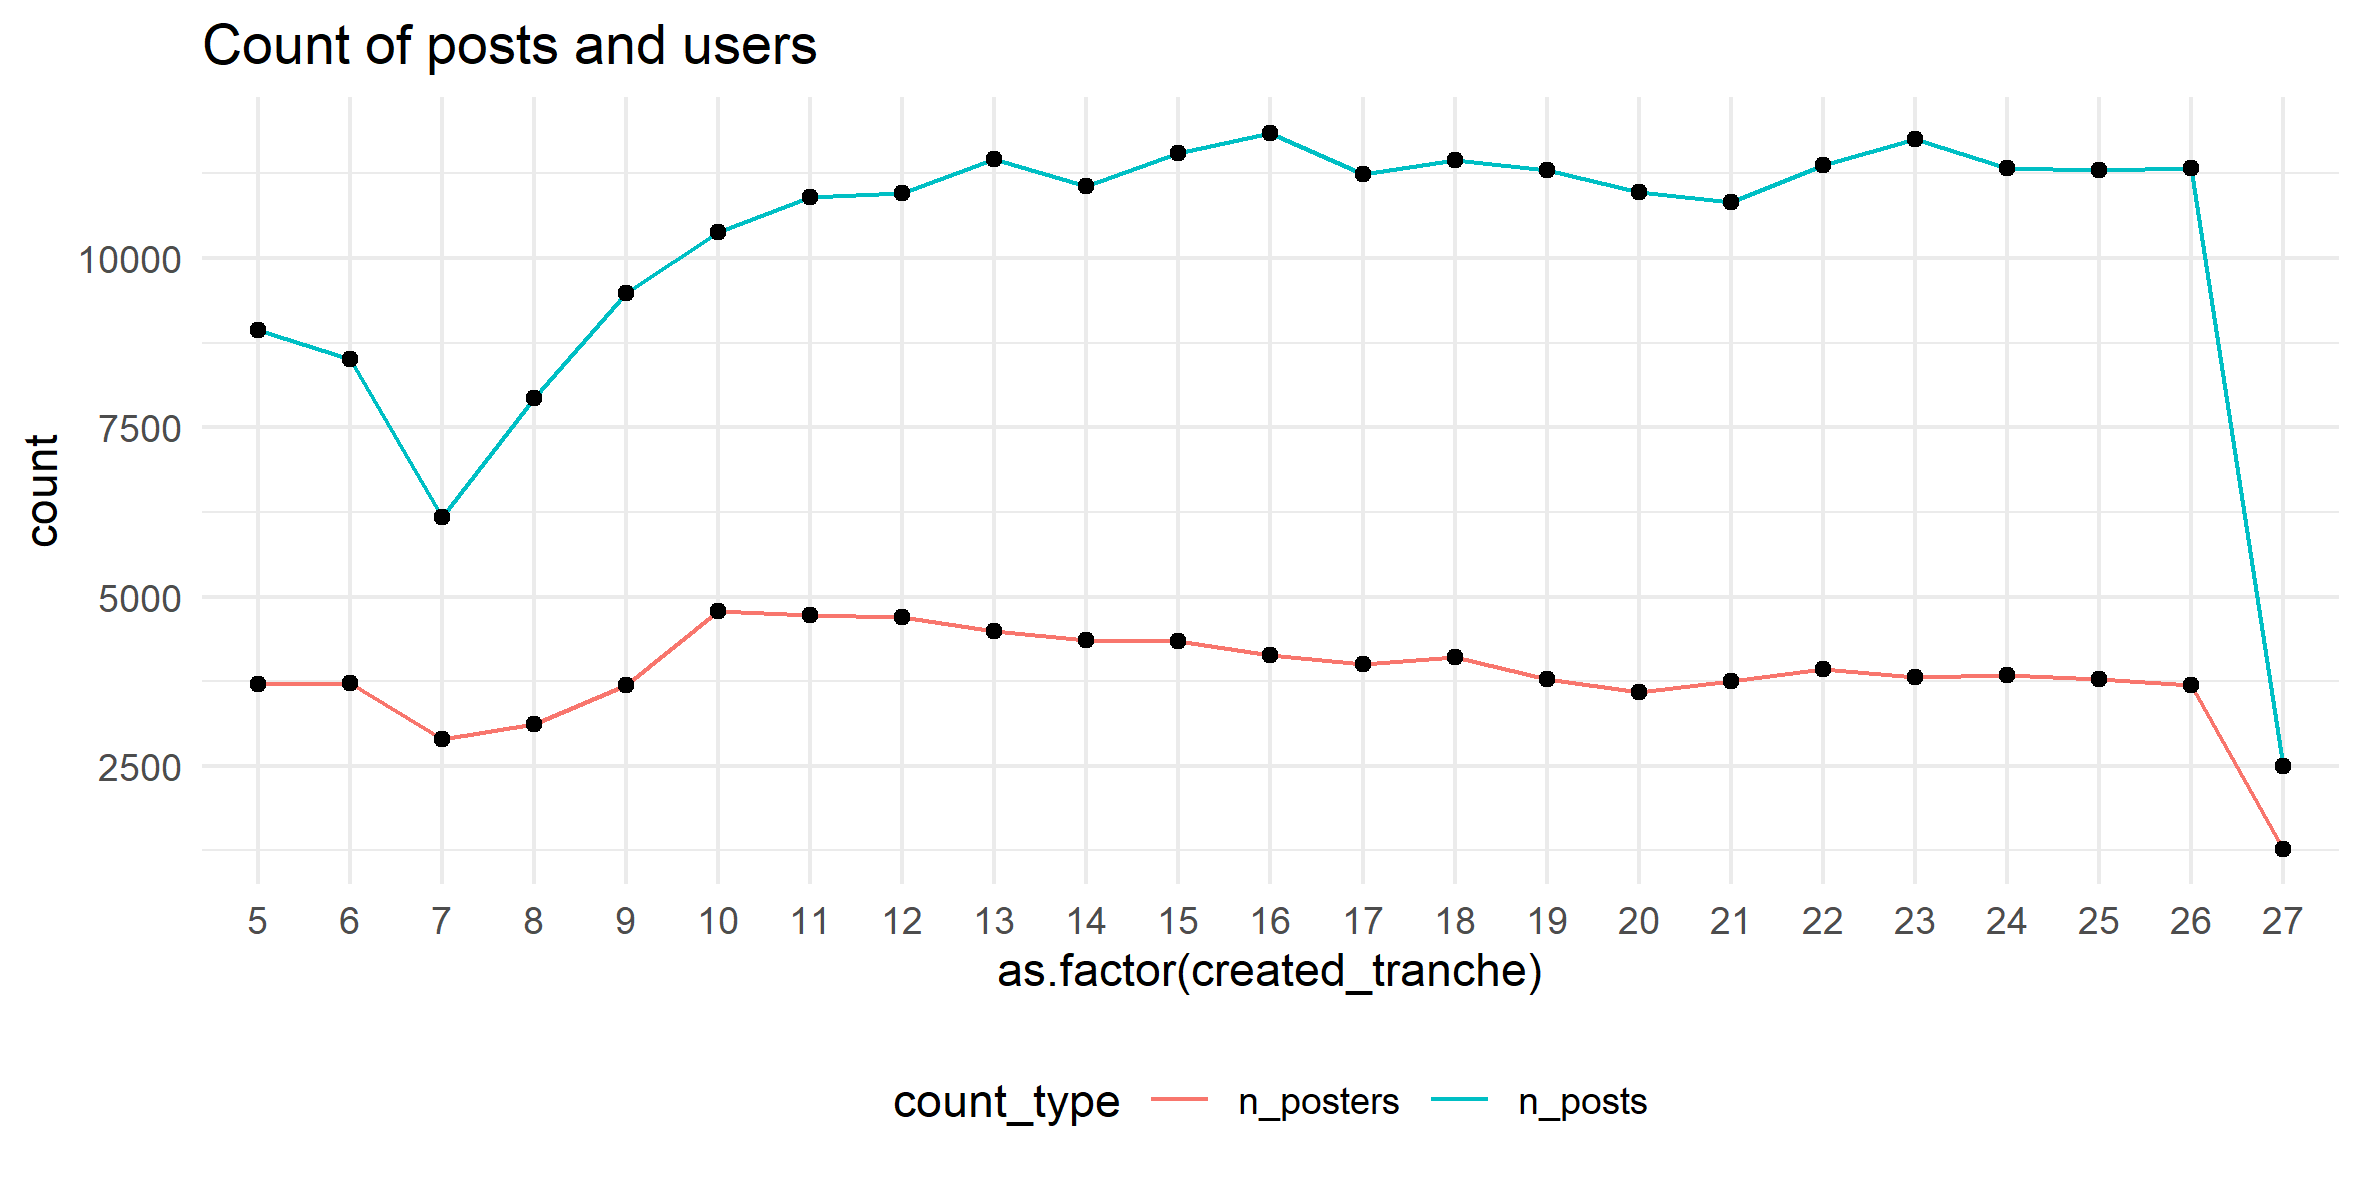
\includegraphics[width=\linewidth]{figures/sub_ts.png}
    \caption{Count of posts and posters for Snapshot Language Models.}%

    \label{fig:sub_stats}%

\end{figure}

% \subsection*{Identifying Elite-users}

% To identify elite users in each window of the subreddit, I construct an interaction network of users. This is the graph of users who have replied to each other, and is constructed from all posts and comments for a given window. It is important to note that only direct replies are considered as a form of interaction. That is, if user B replies to A, and C replies to B, the constructed graph would be:

% \begin{figure}[h]
% \centering
% 
\includegraphics[width=0.5\textwidth]{figures/int_graph.png}
% \caption{Sample Interaction Graph}
% \end{figure}

% The interaction graph is a directional network and weighted by the number of interactions between two users. Elite users for each window are identified using Bonacich centrality, which measures status within the network \citep{bonacich_power_1987}. I examine the top $0.1\%$ of users.

\subsection*{Word Embeddings to describe Context \& Change in Community Discussions}

To describe the context surrounding topics of interest in the community, I construct word embedding models for each period using skip-grams with negative sampling using Python's \texttt{gensim}\citep{rehurek_lrec} library. The high-dimensional corpus of text is reduced to lower dimension where each word $w_i$ is represented by a vector $\textbf{w}_i$ of size $k$ \citep{kozlowski_geometry_2019}. The skip-gram approach captures the nature of co-occurence between words and phrases. Semantic similarity -- and divergence, by extension -- between two words is measured using the cosine similarity between the two word vectors representing them \citep{hamilton_diachronic_2018}. I retain all posts and comments for this method.

To compare the divergence of words from different time-periods, we need to ensure that the word vectors are aligned to the same coordinate axes. I use the Procrustes alignment method developed by Hamilton et al.  \citep{hamilton_diachronic_2018}. For $p$ time-periods, we take the common vocabulary across these periods and obtain the optimal rotational alignment that preserves cosine similarities. After alignment, we can use the adjusted word vectors to compute semantic divergence, i.e. how the context of a word has shifted over time. This is measured using the cosine distance between the word vectors in time $t, t + \Delta$: $cosineDist(\textbf{w}_t, \textbf{w}_{t+\Delta})$. \citep{hamilton_diachronic_2018}

Additionally, I construct semantic dimensions for issues to track how certain the context surrounding specific issues shift over time. For each dimension, I take the normalized sum of antonym pairs to create a bi-directional vector to project word vectors onto. \citep{kozlowski_geometry_2019} The cosine-similarity of word vectors with these dimensions tells us where the word lies on the spectrum created by that dimension. 

I create six dimensions of interest, which are enumerated below. The complete list of antonym pairs used to construct them is provided in Table \ref{tab:dim-table}.

\begin{enumerate}
    \item Security: How closely do entities relate to issues of safety and security. Eg: Are candidates \textit{strong} or \textit{weak} on crime?
    \item Trade: To capture the context around trade issues -- \textit{local} protectionism vs. \textit{global} free trade.
    \item Ideology: Create a dimension to quantify the ideological spectrum between \textit{left} and \textit{right}, \textit{conservative} and \textit{liberal}.
    \item Region: Are the issues of the party focused on cities and the \textit{coast}, or are they referring to the \textit{heartland}?
    \item Economy: Is the party associated with the \textit{rich} and the elite, or do they speak to the \textit{poor} in America.
    \item Race: Where are candidates positioned on questions of race and immigration.
\end{enumerate}

Additionally, I restrict my analysis of these semantic dimensions to four distinct windows. This is to simplify the attempt to explain sifts within the same dimension driven by events. These windows are selected to indicate vital time periods in the Trump presidency. These periods include:  
\begin{enumerate}
	\item Super Tuesday, March 2016: A major victory for Donald Trump in the Republican Primary in key states on Super Tuesday, which made him the front-runner for the nomination. In the run-up to Super Tuesday, he moved from being an outside candidate to a viable candidate, fleshing out his policies and campaign rhetoric.

	\item General Elections, November 2016: Donald Trump beats Hillary Clinton in an upset victory by the slimmest of margins. Coverage in the final days was heavily influenced by investigations into Clinton's e-mail server, precipitated by a letter from FBI director James Comey to Congress about newly discovered material days before the election. 

	\item The first quarter of the presidency, February - March 2017.  

	\item `Unite the Right' rally in Charlottesville, Virginia, August 2017: This was a white-supremacist rally conducted in response to the removal of Confederate monuments by local governments. The rally served as a unifying event for the American white-nationalist movement, and attracted counter-protestors. It turned violent after clashes between the two groups, and on Day 2, a white supremacist deliberately drove his car into the counter-protestors, killing one of them. 
\end{enumerate}  

\begin{table}[t]
\caption{Antonym pairs used to construct Semantic Dimensions}
\label{tab:dim-table}
\resizebox{\textwidth}{!}{%
\begin{tabular}{@{}llrlll@{}}
\toprule
Security & Trade & Ideology & Region           & Economy       & Race         \\ \midrule
safe - vulnerable & local - global & right - left           & rural - urban & rich - poor      & white - black        \\
strong - weak     & tariff - free  & conservative - liberal & town - city   & advantage - need & american - immigrant \\
         &       &          & interior - coast & equity - loan & close - open \\ \bottomrule
\end{tabular}%
}
\end{table}

%------------------------------------------------

\section{Results}

\subsection*{Surprising Language and User Behavior}

The distribution of cross-entropy for each period is fairly similar -- we notice each distribution is fat-tailed and the mean cross-entropy is stable. Period 10, the month of the election, has the highest average cross-entropy. There does not seem to be any variation with time. From Figure \ref{fig:ce_stats}, we also notice that there is no relationship between the cross-entropy and score of a post, and that the relationship between cross-entropy and the number of comments is weak. Thus, filtering on these two parameters would not be equivalent to selecting on the outcome. 

To understand the influence of top users, I plot the average cross-entropy of their posts against that of the community in  Figure \ref{fig:ce_comp}. Top users are defined as those who have made at least 5 posts per period, and whose posts have a mean score greater than 2500 -- regular users whose posts get consistently high scores, about the top 3\% of posters and 10\% of posts. We notice that the cross-entropy of these top users is highly correlated to that of the community at every period, indicating they do not have wildly different language usage from the community. Additionally, we observe that the average cross-entropy of these users is less than the average of the community, i.e. their language is less surprising. This could be an indicator that these users embody the norms of the community, and are thus able to command attention. 

% Cross-Entropy Distribution
\begin{figure}[h]%

    \centering

    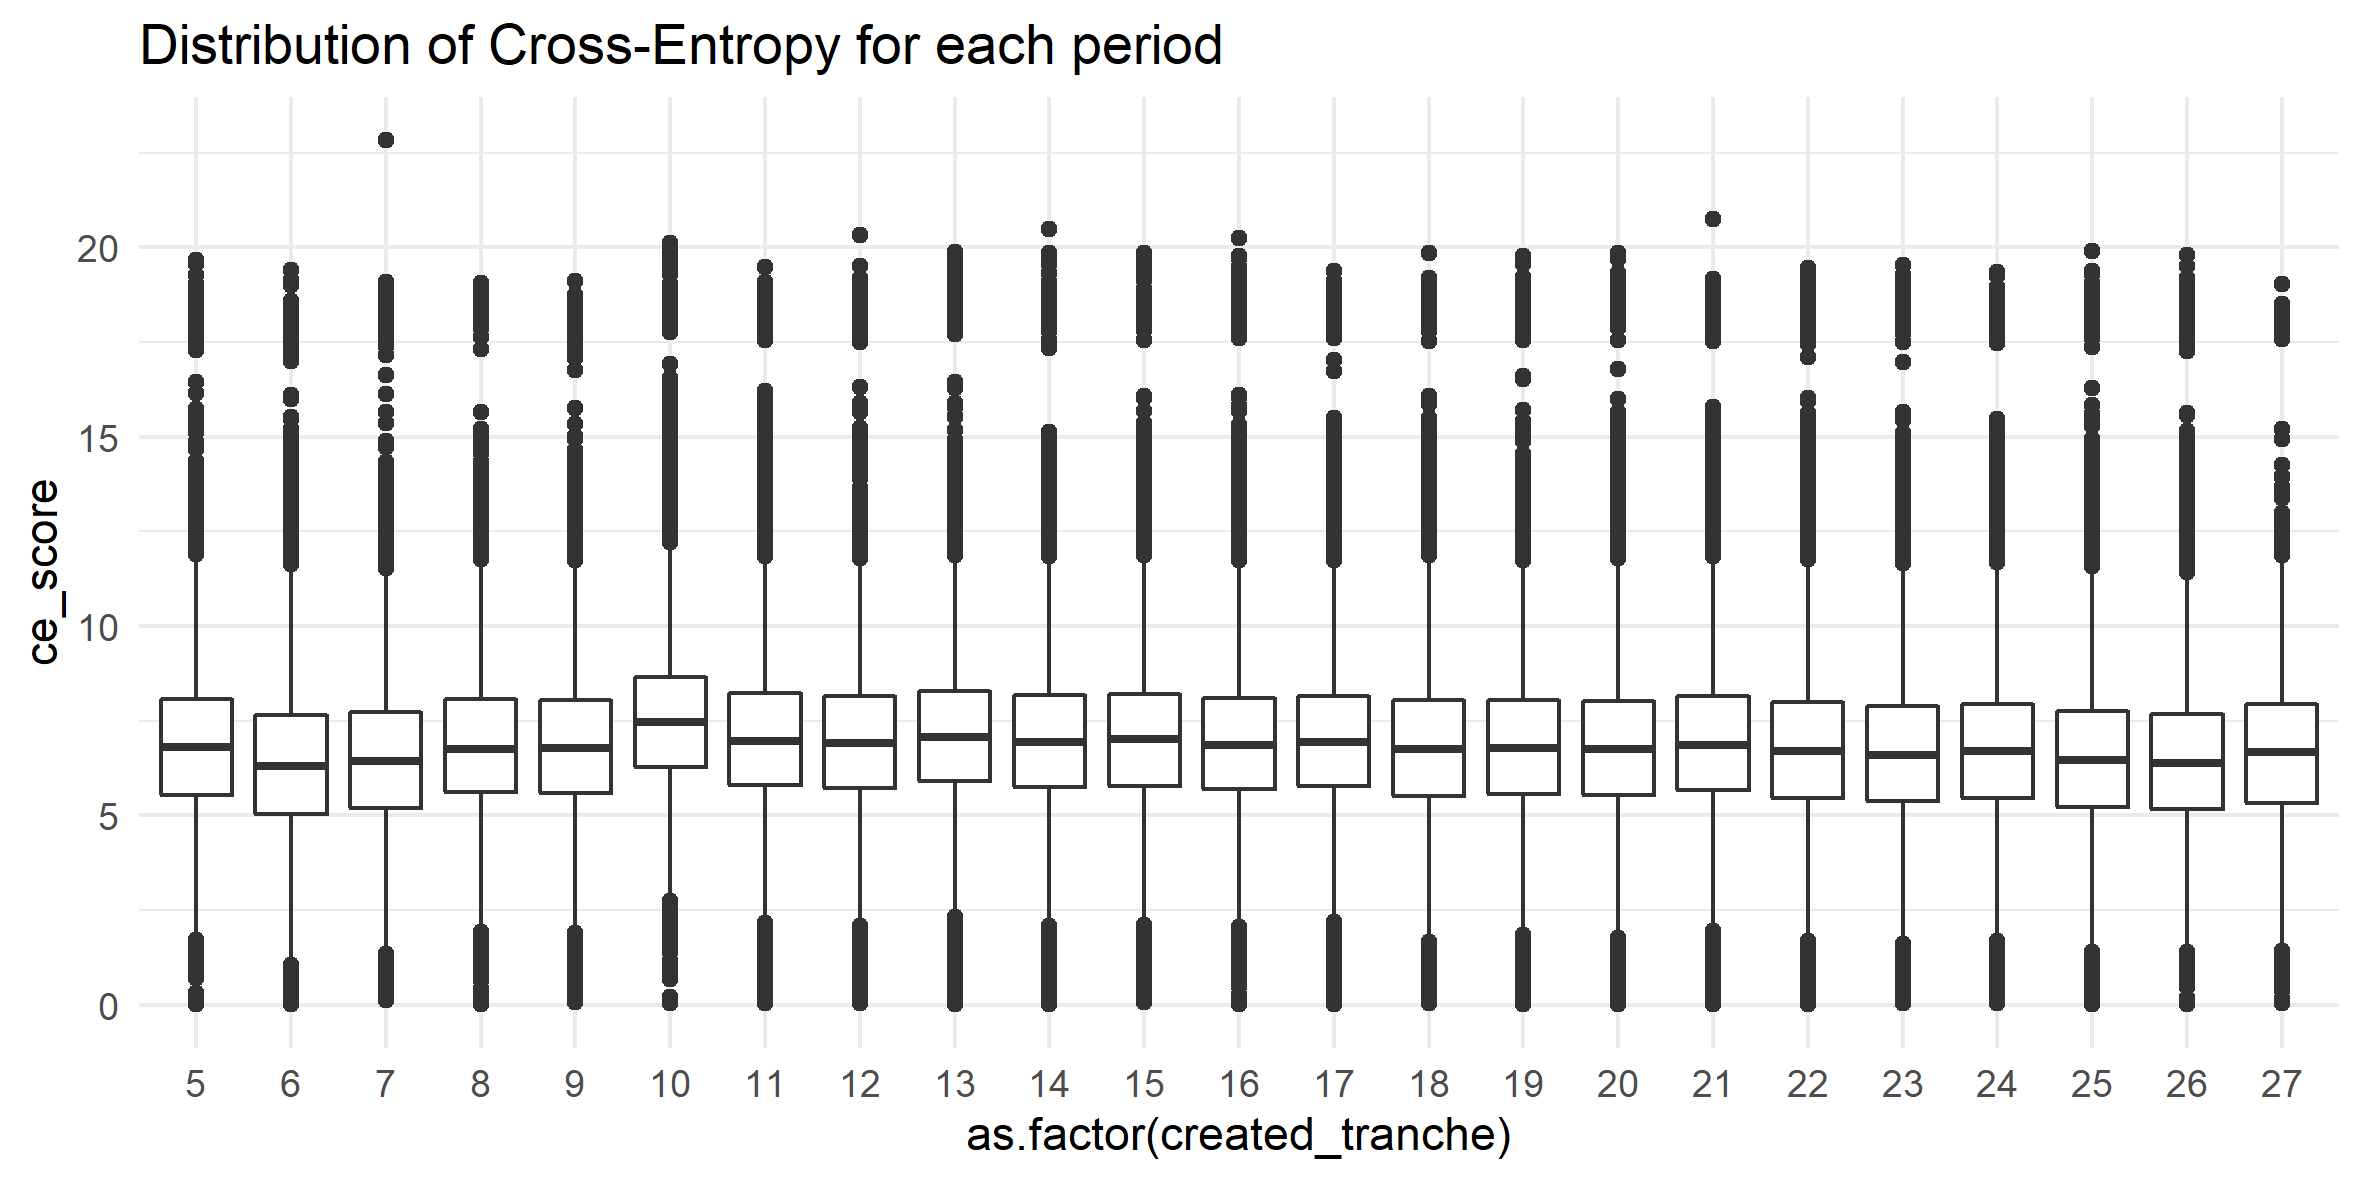
\includegraphics[width=0.8\linewidth]{figures/ce_boxplot.png}
    \caption{Distribution of Cross-Entropy for each 6-week period.}%

    \label{fig:ce_boxplot}%

\end{figure}

% Entropy vs score and comments
\begin{figure}[h]%

    \centering

    \subfloat[Entropy-vs-Score]{{ 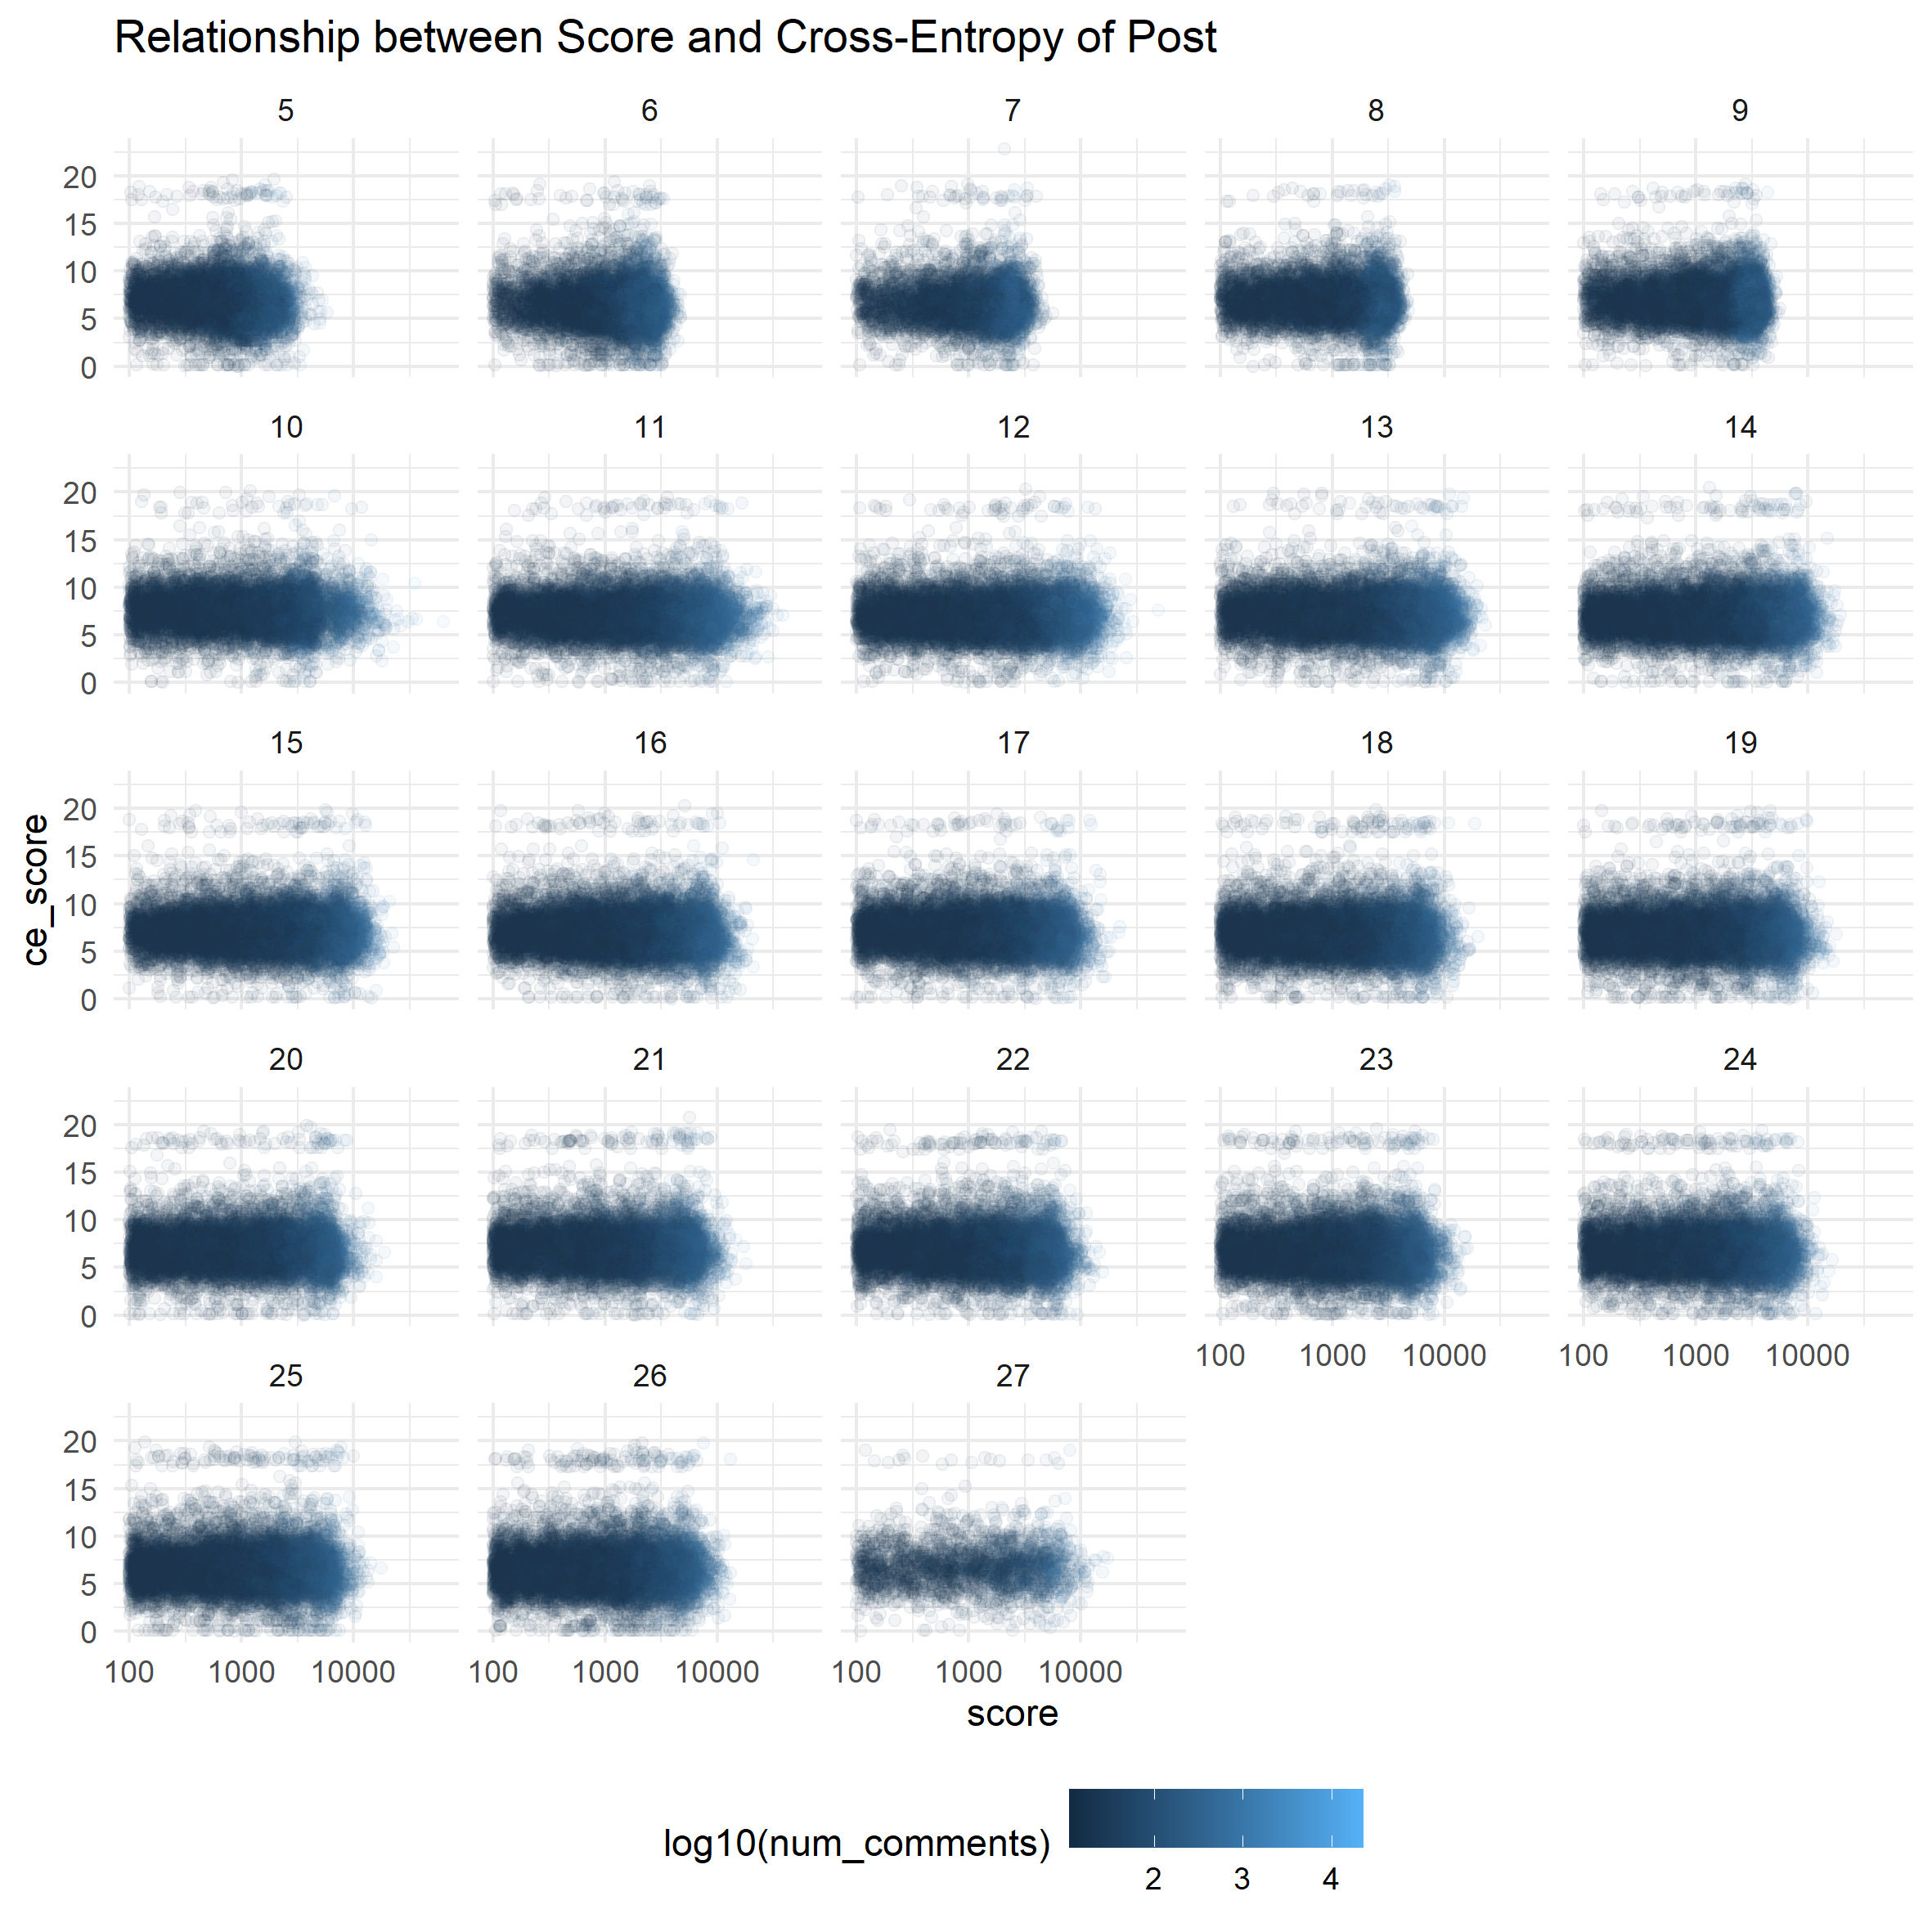
\includegraphics[width=0.45\linewidth]{figures/score_ce_plot.png}}} ~
    \subfloat[Entropy-vs-Comments]{{ 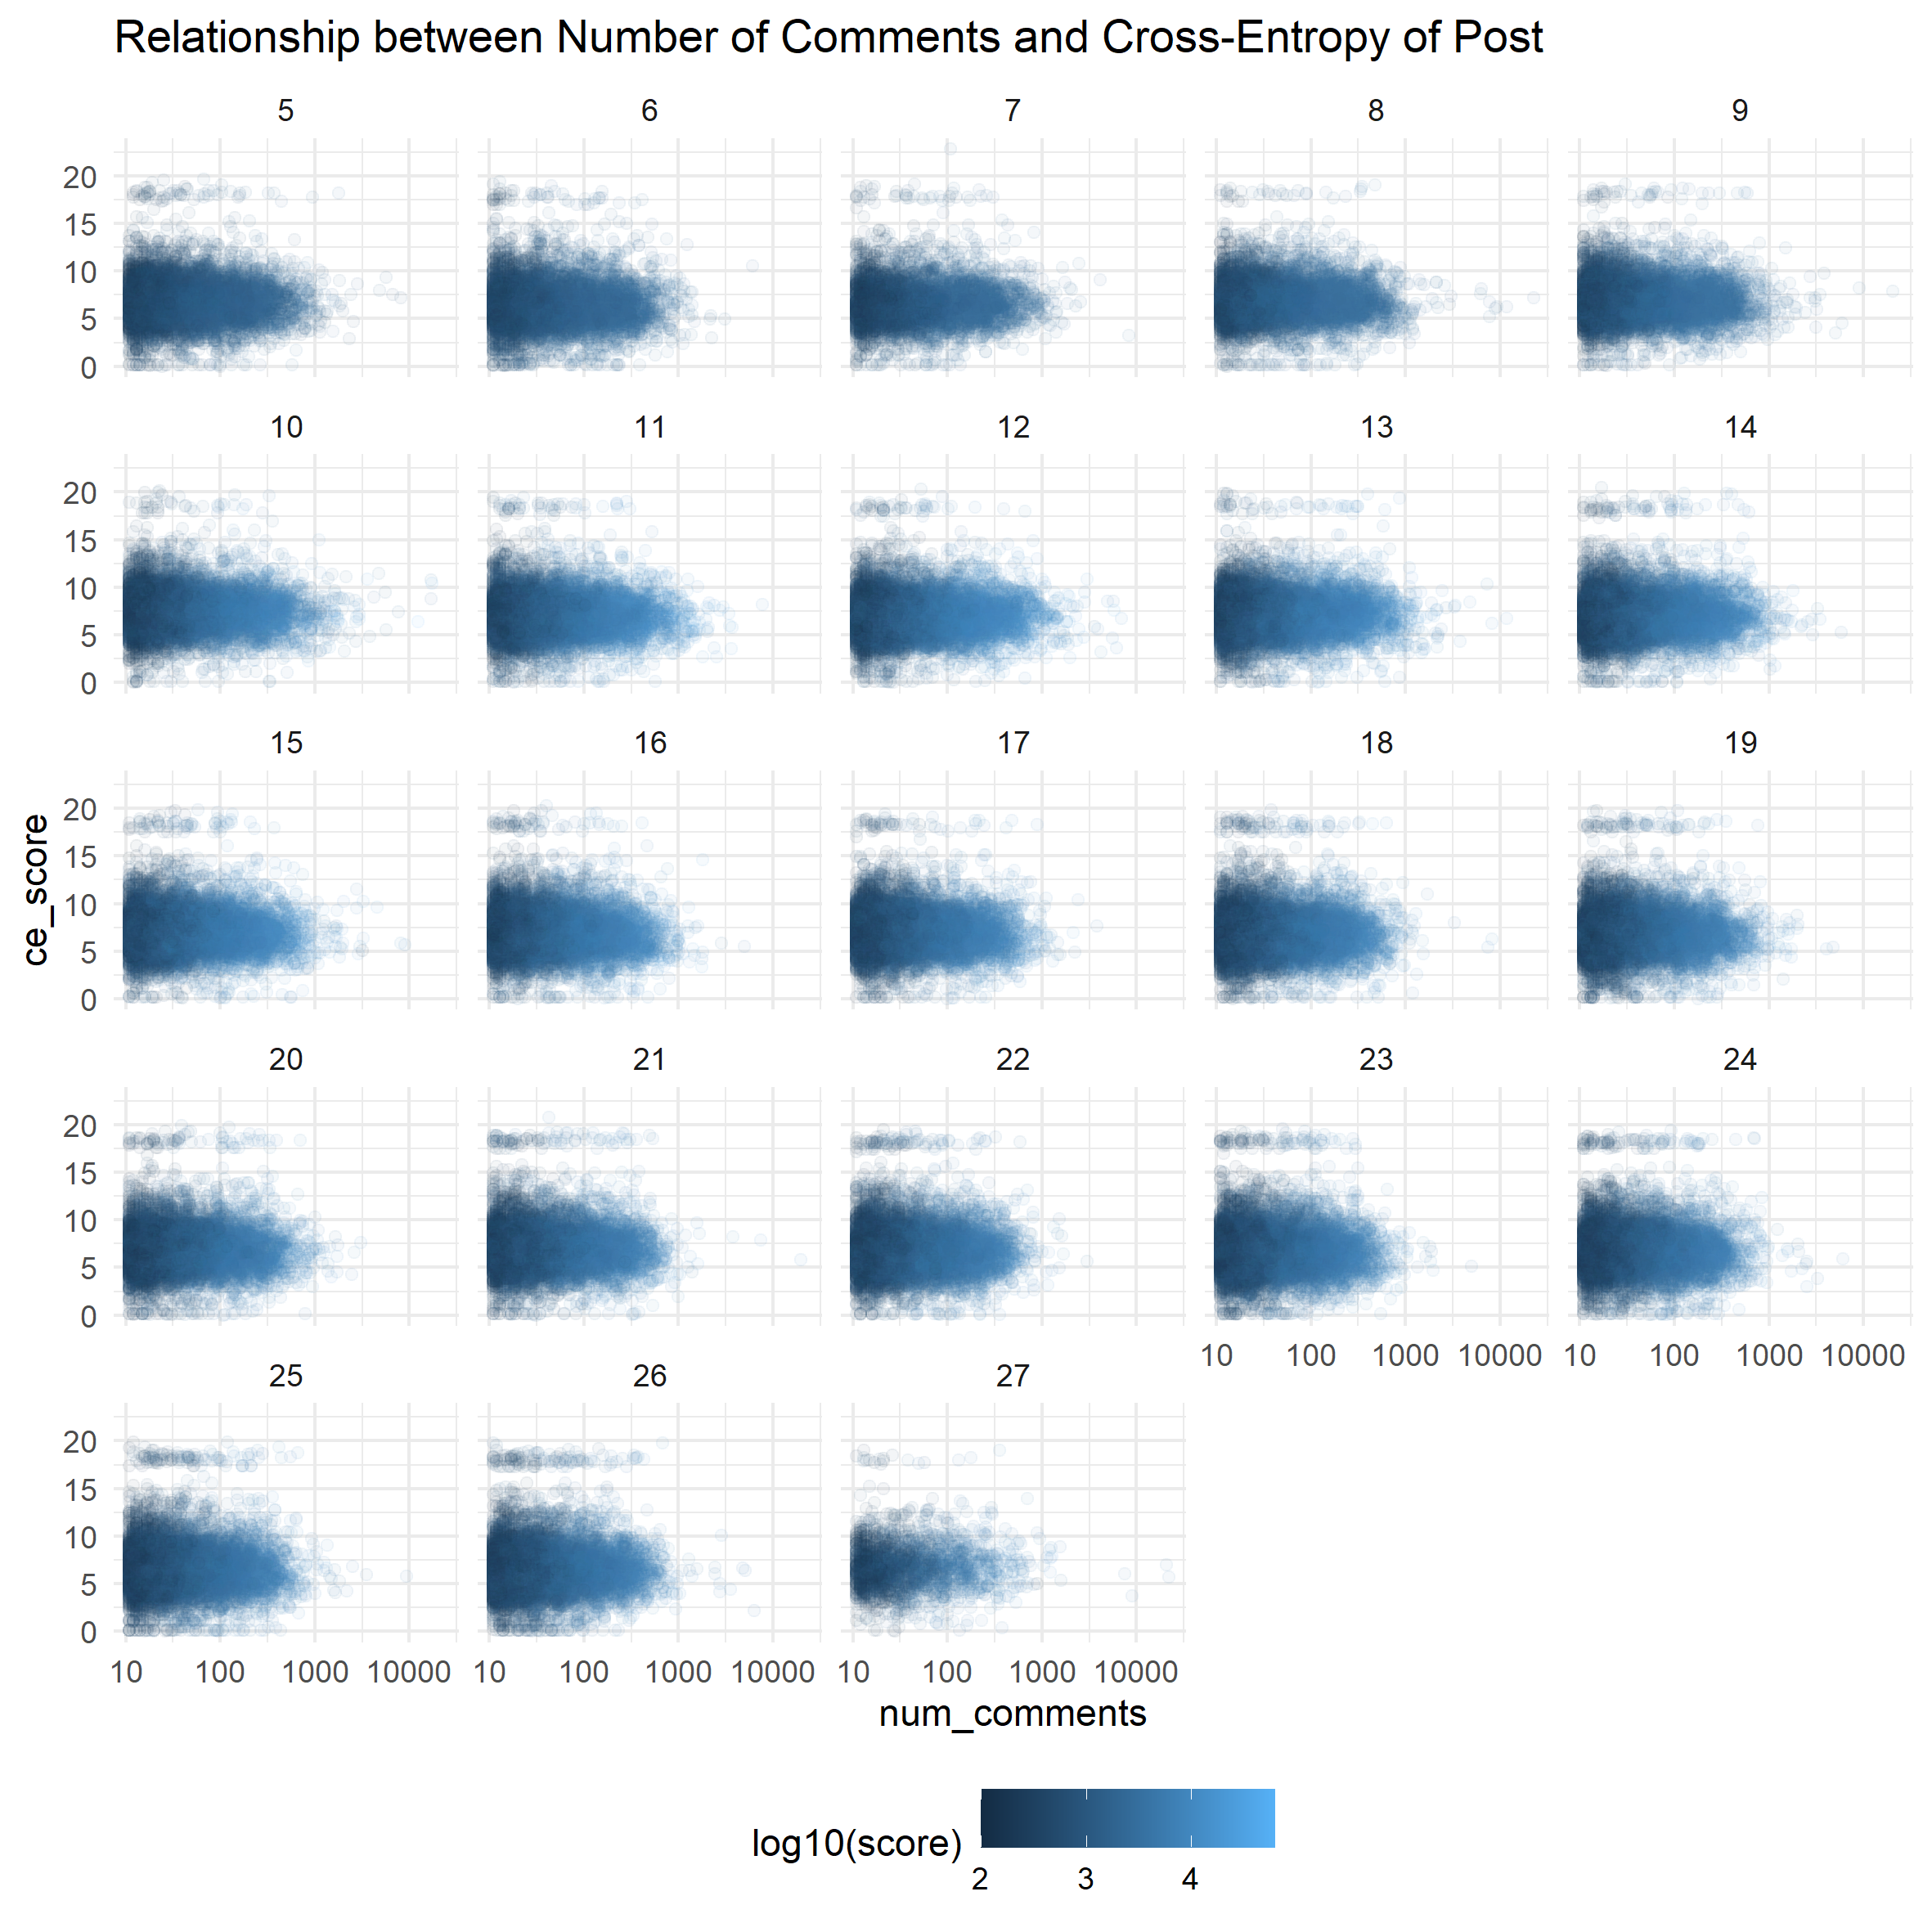
\includegraphics[width=0.45\linewidth]{figures/comm_ce_plot.png} }}
    
    \caption{Relationship between Cross-Entropy and Score, Number of Comments.}%

    \label{fig:ce_stats}%

\end{figure}


% Cross-Entropy of top-users
\begin{figure}[h]%

    \centering

    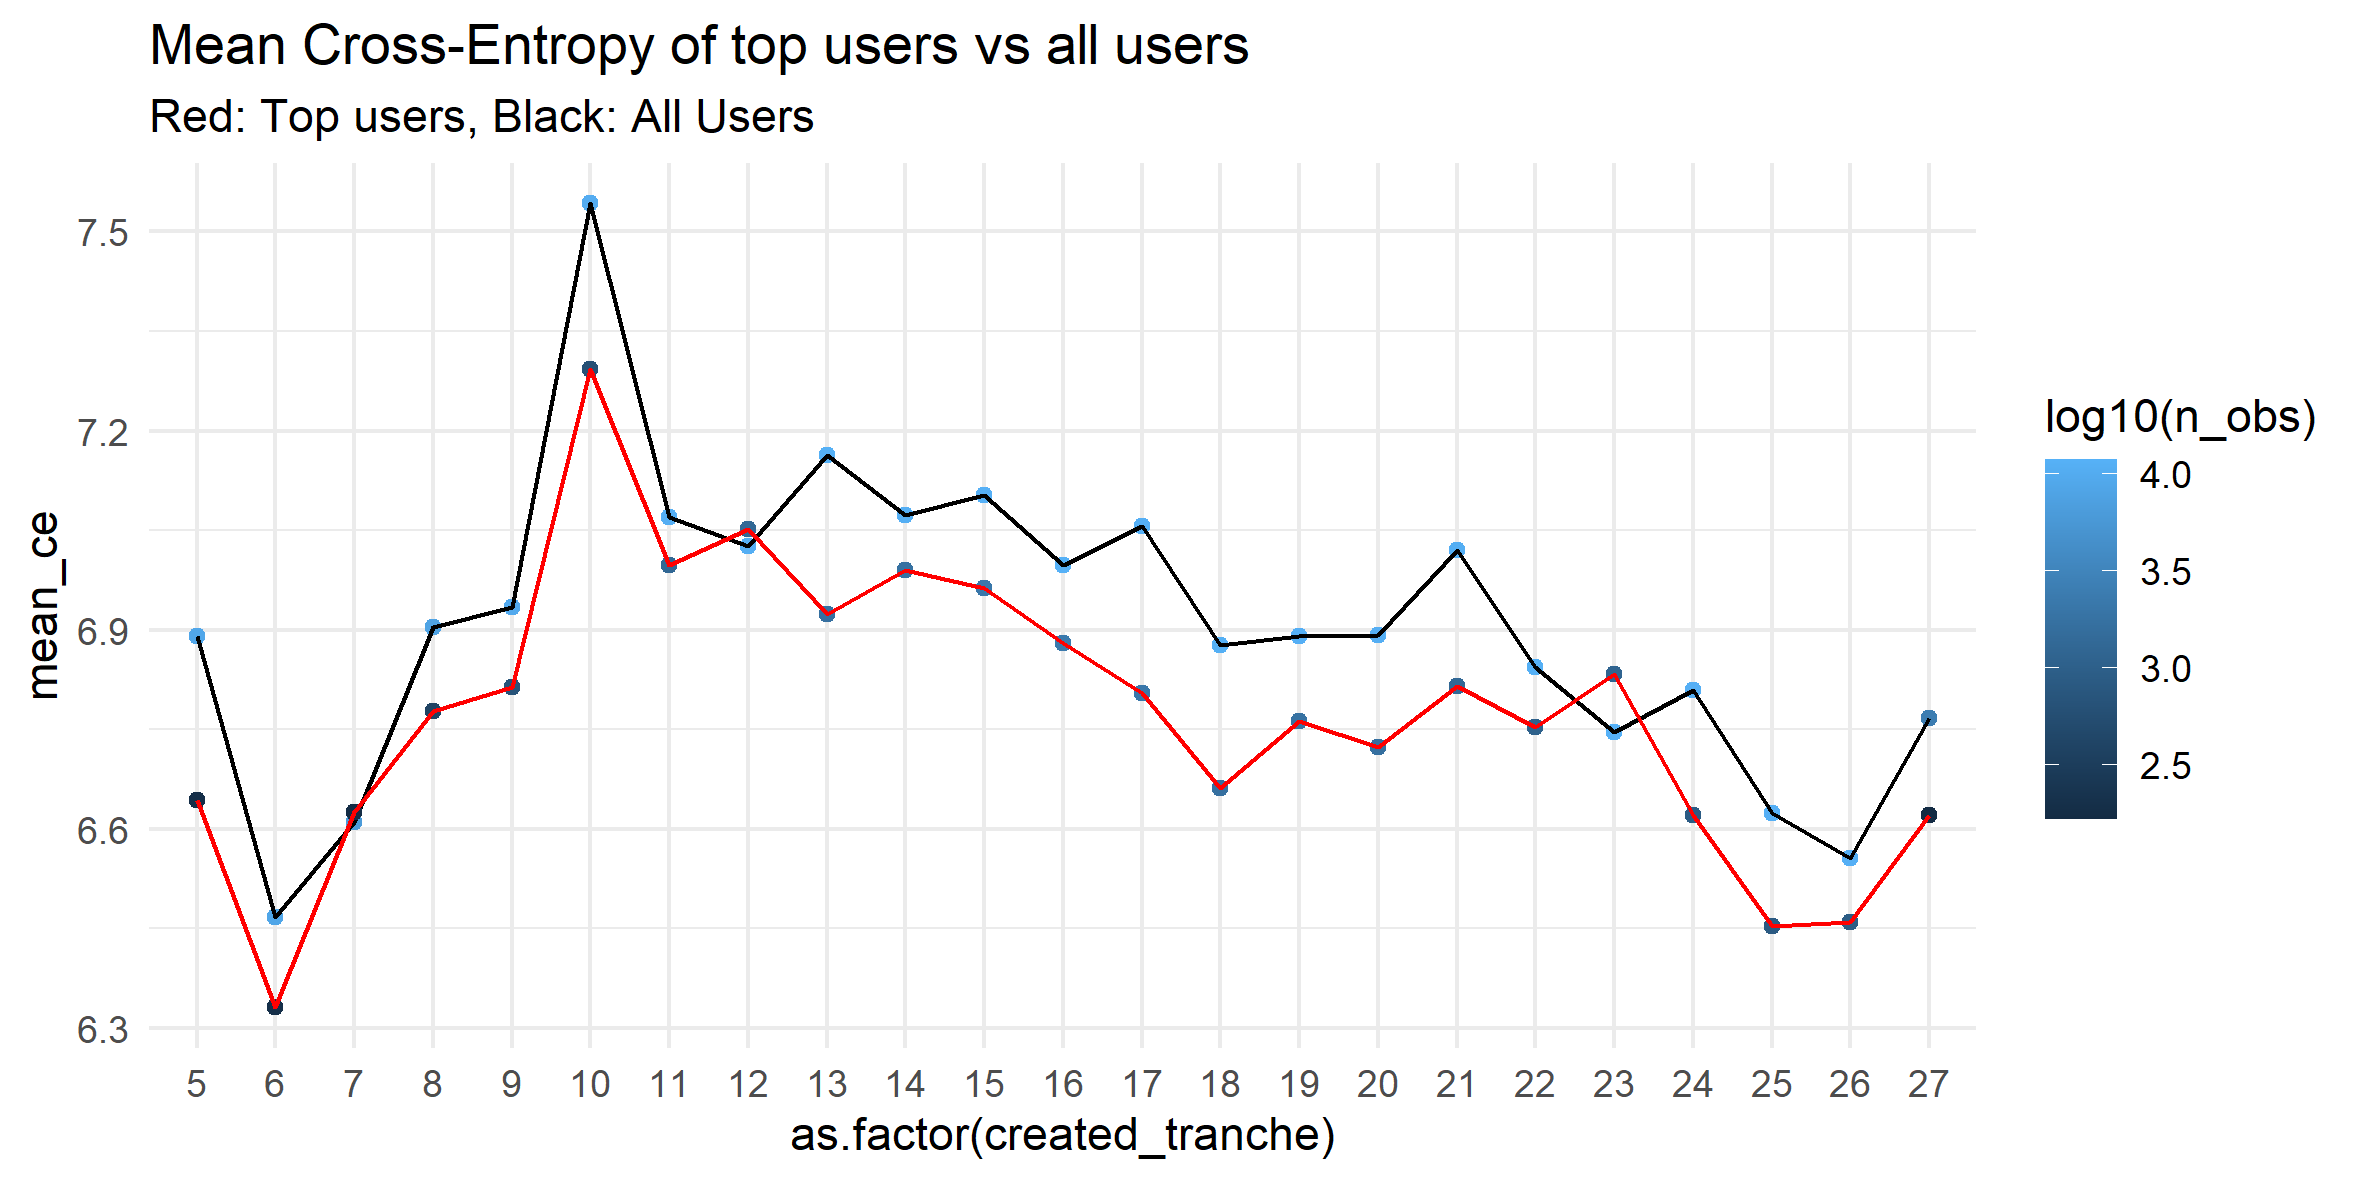
\includegraphics[width=\linewidth]{figures/comp_ce_plot.png}
    \caption{Mean Cross-Entropy of all posts vs top users for each 6-week period.}%

    \label{fig:ce_comp}%

\end{figure}



\clearpage
\subsection*{Using Divergence measures to identify a change in context}

\subsubsection*{Immigration policies}

% Divergence of Immigration
\begin{figure}[t]%

    \centering

    \subfloat[`immigrant']{{ 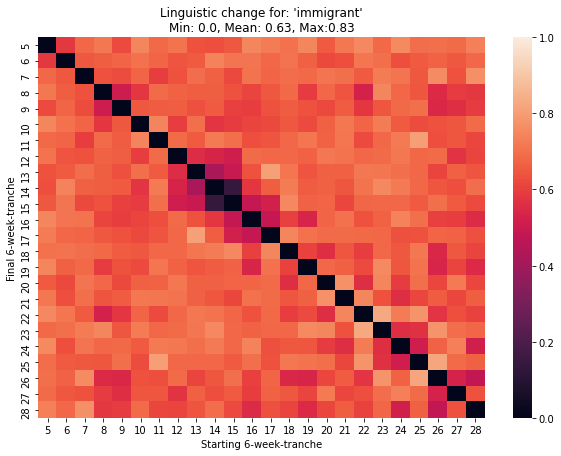
\includegraphics[width=0.32\linewidth]{figures/div_graphs/immigrn-immigrant.png} }} ~
    \subfloat[`border']{{ 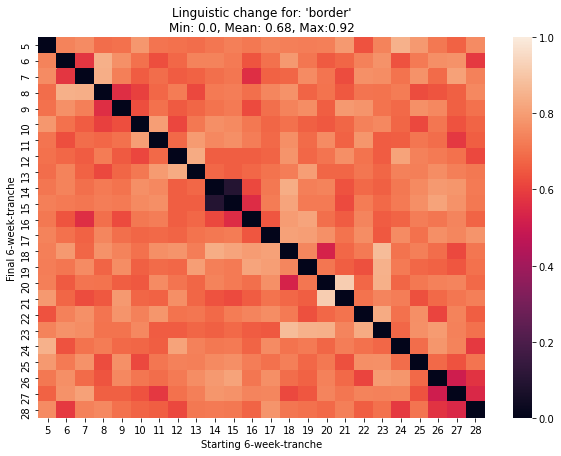
\includegraphics[width=0.32\linewidth]{figures/div_graphs/immigrn-border.png} }} ~
    \subfloat[`separation' (Family Separation policy)]{{ 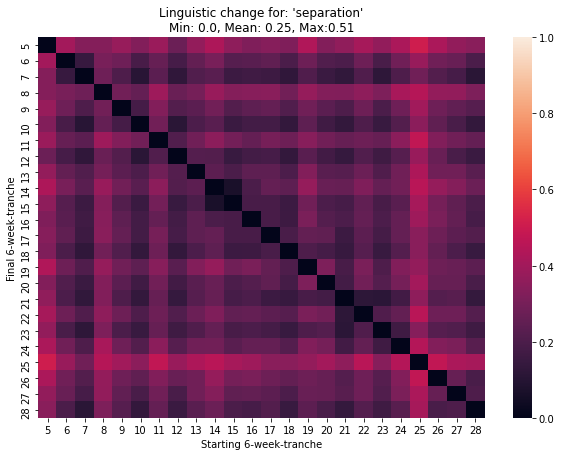
\includegraphics[width=0.32\linewidth]{figures/div_graphs/scandal-separation.png} }}
    
    \subfloat[`hispanic']{{ 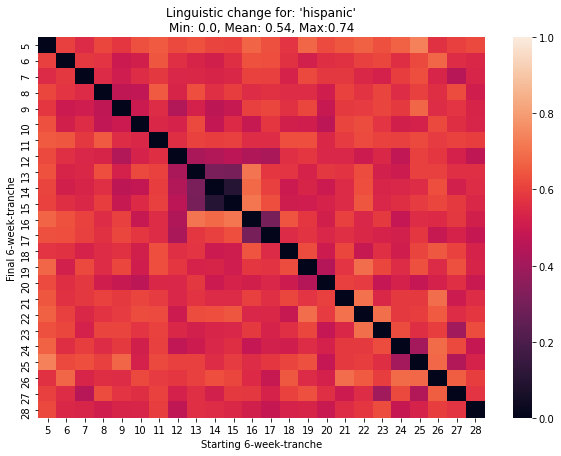
\includegraphics[width=0.32\linewidth]{figures/div_graphs/immigrn-hispanic.png} }} ~
    \subfloat[`mexican']{{ 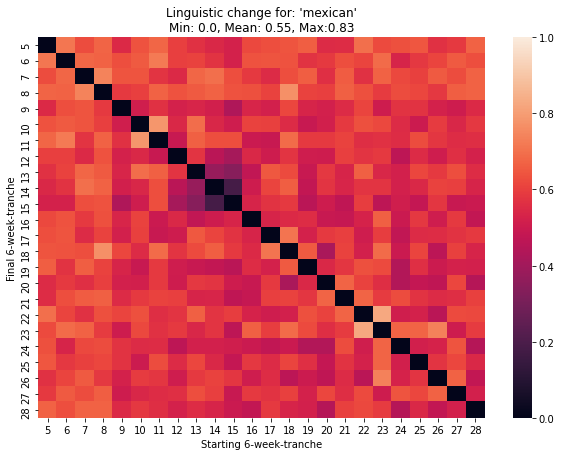
\includegraphics[width=0.32\linewidth]{figures/div_graphs/immigrn-mexican.png} }}~
    \subfloat[`muslim']{{ 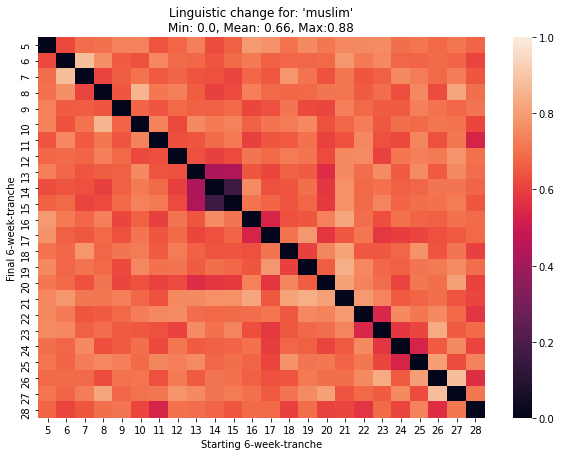
\includegraphics[width=0.32\linewidth]{figures/div_graphs/immigrn-muslim.png} }}
    
    \caption{Relative Divergence of words related to Trump's Immigration policies using aligned word embeddings.}%

    \label{fig:div_immigr}%

\end{figure}

Immigration was and continues to remain a cornerstone of President Trump's legislative agenda. The first notes of stabilization for \texttt{immigrant, border} begin in period 12 in the early months of the presidency, as we see in Figure \ref{fig:div_immigr}. The thrust on immigration continues until period 17, before it picks up again during periods 22. This later spike is associated with the legislative focus on the border family separation issue. The community's context around \texttt{separation} changes in period 25 -- when President Trump signed the executive order rescinding the Family Separation policy \citep{noauthor_family_nodate}. 

The focus on immigration translates into increased attention on ethnic and religious minorities. There is a notable change in the use of \texttt{mexican} right after the election, with an associated and muted change in \texttt{hispanic} a few periods later, with both stabilizing in the same periods as above. I expected to see a related uptick in \texttt{muslim} in association to President Trump's Muslim ban \citep{noauthor_timeline_2017}. The ethno-nationalist focus of the subreddit's ideology creates confounders in contextualizing the word.
%--------------------------------------------------------%

\subsubsection*{References to news media}

% Divergence of news
\begin{figure}[t]%

    \centering

    \subfloat[`cnn']{{ 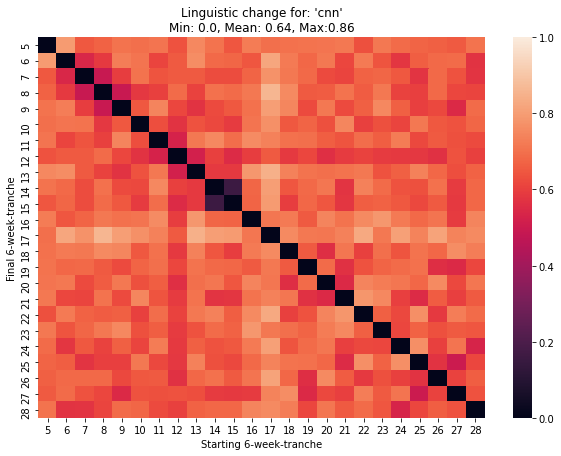
\includegraphics[width=0.32\linewidth]{figures/div_graphs/news-cnn.png} }} ~
    \subfloat[`fox']{{ 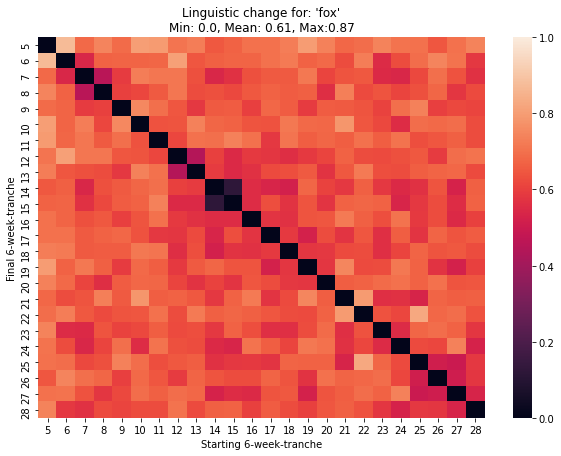
\includegraphics[width=0.32\linewidth]{figures/div_graphs/news-fox.png} }}~ 
    \subfloat[`breitbart']{{ 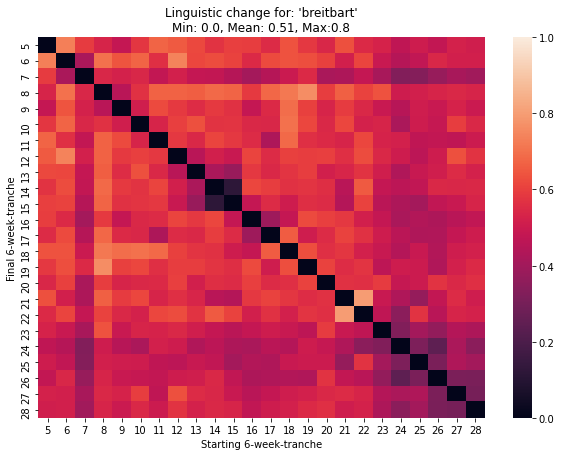
\includegraphics[width=0.32\linewidth]{figures/div_graphs/news-breitbart.png} }}
    
    \caption{Relative Divergence of names of prominent news outlets using aligned word embeddings.}%

    \label{fig:div_news}%

\end{figure}

A salient highlight of President Trump's term has been his frequent attacks on news media outlets, charging them as the 'enemy of the people', of having a vendetta against him, going so far as to institute a list of 'Fake News' award winners. This messaging has had significant success within his base, furthering a partisan re-framing of institutions and working to de-legitimize them. The multiple and varying references to \texttt{cnn} -- albeit in different contexts, since they report on a multitude of issues -- seem like a strong indicator of their centrality to the conversations in the subreddit. The spike in divergence values in period 17 refer to the incident where President Trump re-tweeted a video of attacking CNN.  

On the other hand, President Trump has also expertly tapped into the right-wing media ecosystem to amplify his message. He has made several announced appearances on talk shows hosted by Fox News to chime in on policy. Steve Bannon, chief editor of Breitbart News, was a key figure in the election campaign and was appointed Chief Strategist after the election win, at par with the Chief of Staff \citep{noauthor_donald_2016}. Breitbart has also been a cornerstone of the alt-right, with its nativist and highly partisan coverage crafted for online amplification, replete with fake news and conspiracy theories. For two important news outlets occupying a similar ideological space, their impressions in the subreddit vary drastically. 

% Divergence of Milo vs Hannity
\begin{figure}[h!]%

    \centering

    \subfloat[`hannity' (Sean Hannity)]{{ 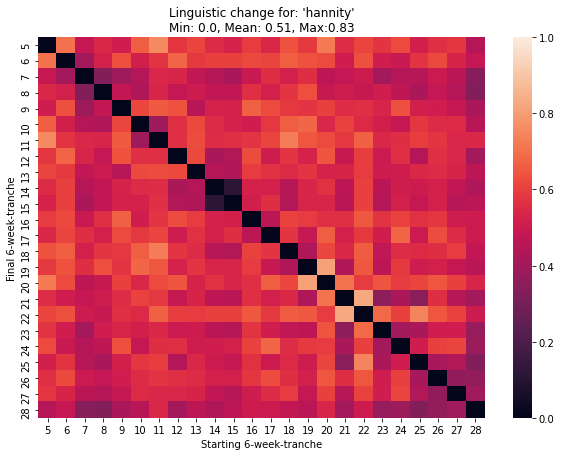
\includegraphics[width=0.32\linewidth]{figures/div_graphs/news-hannity.png} }} ~
    \subfloat[`milo' (Milo Yiannopoulos)]{{ 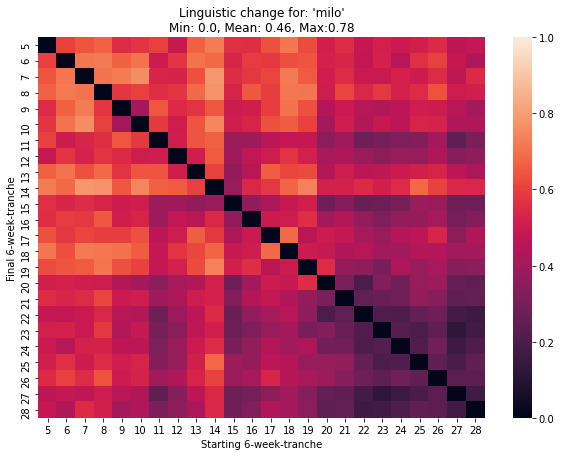
\includegraphics[width=0.32\linewidth]{figures/div_graphs/news-milo.png} }} 
    
    \caption{Relative Divergence of prominent media figures on the right using aligned word embeddings.}%

    \label{fig:div_milo}%

\end{figure}
%--------------------------------------------------------%

\texttt{fox}'s relative divergence map varies in a form similar to that of \texttt{cnn}, while \texttt{breitbart} is likely used in fewer contexts. For the latter, we notice a high change in context at period 22, followed by a period of lower divergence, indicating a stabilization and narrowing of context. The relative fortunes of Fox and Breitbart indicate a shift in attention of the subreddit's sources, with Fox taking on a markedly different role from the first month of the presidency. This shift away from Breitbart is captured well in the subreddit's references to \texttt{milo}, i.e. Milo Yiannopoulos, alt-right provocateur and former editor of Breitbart News. Yiannopoulos's decline as the darling of the alt-right -- following his remarks on pedophilia and child sexual abuse -- tracks with the muted attention of Breitbart in the subreddit, an indicator of weakening influence. 

%--------------------------------------------------------%



\subsubsection*{Salience of Clinton's e-mails and the Russia Investigation}

In Figure \ref{fig:div_emails}, we notice that the term \texttt{email} first changes significance in period 8 and continues to change until period 11. The context stabilizes in periods 16-18. These changes track closely to those of \texttt{russia}, which is to be expected, given Russia's role in the controversy. The timing of these changes coincide with the investigations into Russian interference in the 2016 US elections. These terms both have a high maximum value of divergence, indicating the possibly polysemous nature in which they're being used. The more muted nature of \texttt{hack} is a stronger indicator of the e-mail controversy, owing to its usage in association with the John Podesta email hack. Compared to the use of \texttt{leak} which could refer to other administrative leaks with varying contexts in the Trump government, it has much greater variation in usage. 

Figure \ref{fig:div_scandals} shows us how the context around the impeachment investigations have changed over time. We notice a spike in divergence in period 11 for \texttt{impeach}, right after the election, indicating how this was a hot-button issue immediately. Additionally, we notice a rise in divergence in period 13 for \texttt{hoax}, pointing to President Trump's claims calling Russian interference in the elections a hoax \citep{noauthor_trump_2019}. We see a higher and more disperse spread of divergence for \texttt{hunt}, beginning in period 17, when President Trump claimed that the Democrats were engaged in a 'witch hunt' \citep{noauthor_donald_nodate}. 

% Divergence of scandals
\begin{figure}[h!]%

    \centering

    \subfloat[`impeach' (Impeachment)]{{ 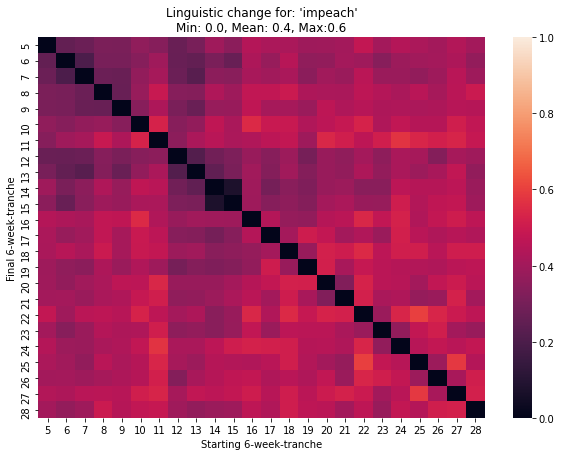
\includegraphics[width=0.28\linewidth]{figures/div_graphs/scandals-impeach.png} }} ~
    \subfloat[`hoax' (Russia hoax)]{{ 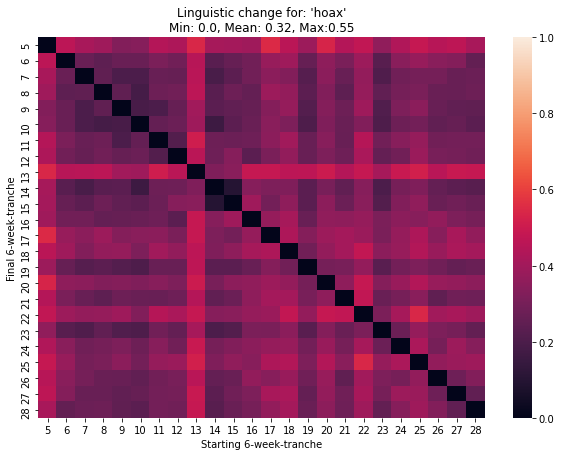
\includegraphics[width=0.28\linewidth]{figures/div_graphs/scandals-hoax.png} }} ~
    \subfloat[`hunt' (`Witch Hunt')]{{ 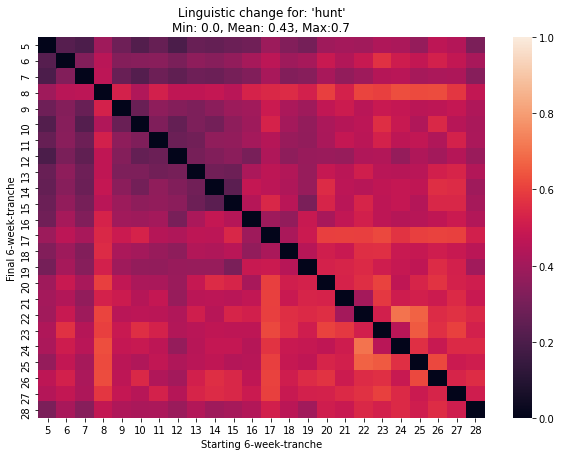
\includegraphics[width=0.28\linewidth]{figures/div_graphs/scandals-hunt.png} }}
    
    \caption{Relative Divergence of words related to Trump's scandals using aligned word embeddings.}%

    \label{fig:div_scandals}%

\end{figure}

% Divergence of e-mails
\begin{figure}[t]%

    \centering

    \subfloat[`email']{{ 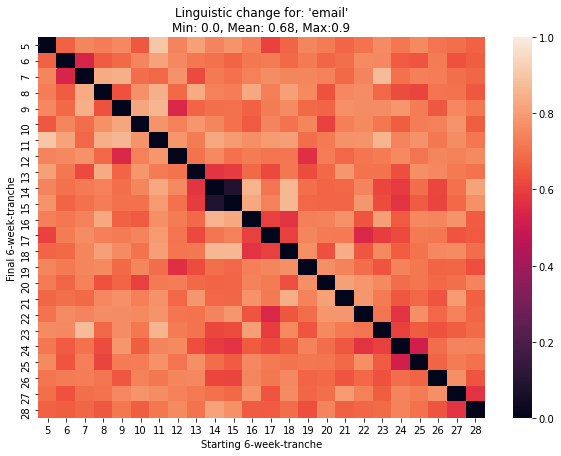
\includegraphics[width=0.28\linewidth]{figures/div_graphs/emails-email.png} }} ~
    \subfloat[`russia']{{ 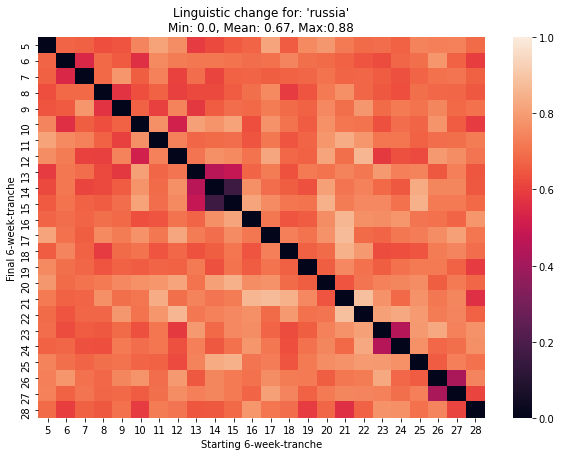
\includegraphics[width=0.28\linewidth]{figures/div_graphs/emails-russia.png} }}
    
    \subfloat[`hack']{{ 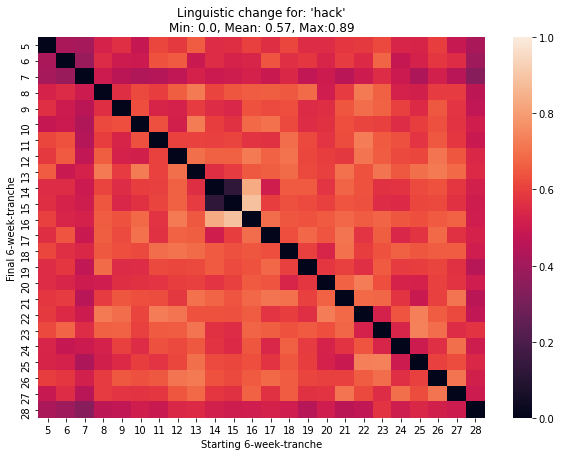
\includegraphics[width=0.28\linewidth]{figures/div_graphs/emails-hack.png} }} ~
    \subfloat[`leak']{{ 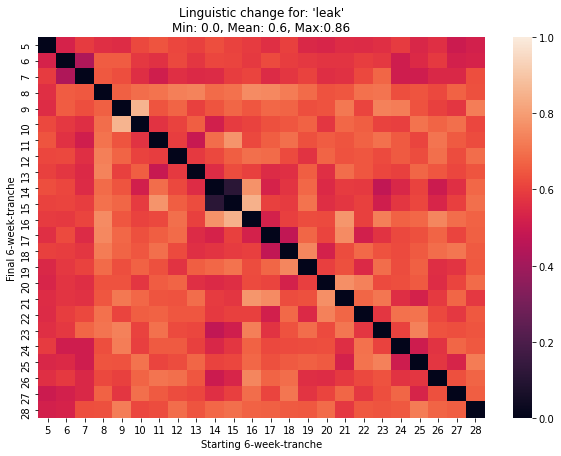
\includegraphics[width=0.28\linewidth]{figures/div_graphs/emails-leak.png} }}
    
    \caption{Relative Divergence of words related to Clinton's e-mail controversy using aligned word embeddings.}%

    \label{fig:div_emails}%

\end{figure}
%---------------------------------------------------------%

\subsubsection*{Tracking tariffs and the trade war}

President Trump's focus on 'Make America Great Again' has also translated into renewed attention on American manufacturing, and the the effect of free-trade agreements on jobs in America. As he tried to publicly push companies to move jobs back to the US, he also criticized past administrations for crafting unfavourable trade deals with China. This soon morphed into a trade war with China, with escalating tariffs levied by both sides.  We notice the first change in the context surrounding the word \texttt{tariff} in period 13, in the first quarter of the presidency, followed by no change for an extended period. This is indicative of a significant change in rhetoric in period 13, until period 23. The change in period 23 is matched by those for words \texttt{trade} and \texttt{china}. This period included a serious escalation of the trade war with China. 

% Divergence of trade
\begin{figure}[b]%

    \centering

    \subfloat[`China']{{ 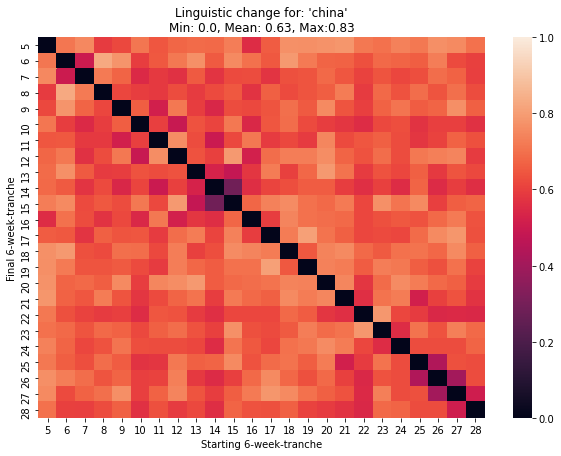
\includegraphics[width=0.265\linewidth]{figures/div_graphs/trade-china.png} }} ~
    \subfloat[`tariff']{{ 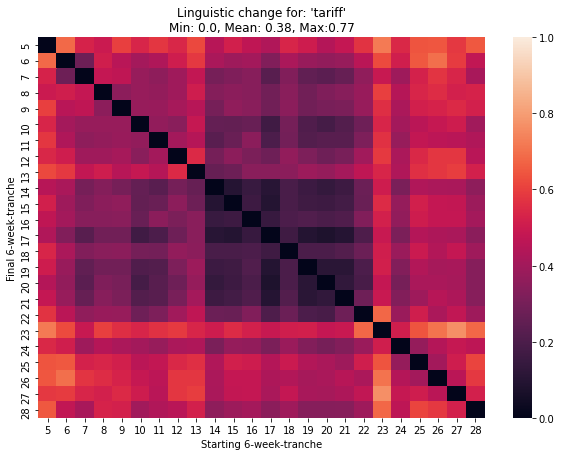
\includegraphics[width=0.265\linewidth]{figures/div_graphs/trade-tariff.png} }} ~
    \subfloat[`trade']{{ 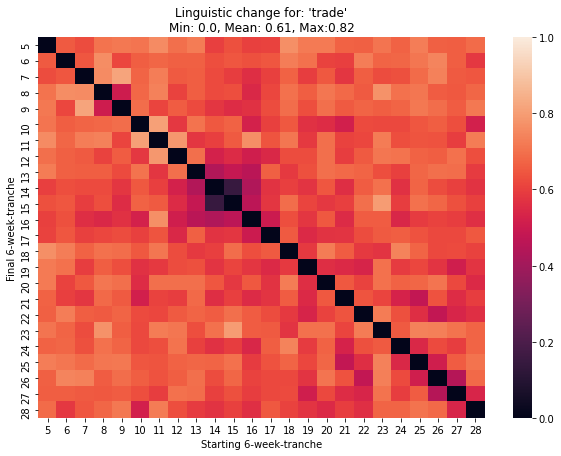
\includegraphics[width=0.265\linewidth]{figures/div_graphs/trade-trade.png} }} 
    
    \caption{Relative Divergence of words related to Trump's trade war with China using aligned word embeddings.}%

    \label{fig:div_trade}%

\end{figure}

%--------------------------------------------------------%


\subsection*{Using Projections of Word Embeddings to understand relative positions}

\subsubsection*{Changing associations of political figures}

Figure \ref{fig:proj_parties} provides a projection of political names and entities onto dimensions of security, trade, ideology, region, economy, and race. I select the names of the candidates in the 2016 US elections and the names of the political parties, to understand how their relative positions on these political dimensions change over time in the subreddit. This helps us understand how the community's language and context around these figures, and by extension their perception of these entities, has shifted over time. 

On the `Security' dimension in figure \ref{fig:proj_parties}, we notice how \texttt{trump} ranks consistently high relative to all other entities. \texttt{clinton} moves towards the lower end of the dimension in the month of the election, indicating how the subreddit viewed her as being weak on Security issues. \texttt{democrat} is consistently on the lower dimension (weak security) in all but one window, that of the election. I interpret this as Clinton's fall from relevance as the opposition to President Trump after his election. 

On questions of Ideology, we notice \texttt{trump} and even \texttt{democrat} not being fixed on the dimension, with only \texttt{republican} being static. We also notice how \texttt{bernie} and \texttt{stein} consistently represent the opposite of the Republican ideology. This latter observation should not be surprising -- Bernie Sanders and Jill Stein have been purists for the duration of their political careers, and stand in stark opposition to the Republicans. Interestingly, in the  period of the election, \texttt{stein} moves to the center while \texttt{clinton} moves to the extreme -- a strong indicator of how perceptions in the lead-up to the elections were vastly different from other periods.

On questions of the Economy, \texttt{trump} loads heavily on the poor or non-elite end of the dimension, affirming the perception of his anti-establishment credentials.  \texttt{bernie} occupies a similar position. \texttt{clinton} is positioned on the `rich' end of the dimension in the month of the election, showcasing how her established pedigree came to the fore in that period. On the dimension of Race, \texttt{trump} shows up close to the extreme in two windows: Super Tuesday 2016, and August 2017 during the Charlottesville attack. Both these periods were dominated by strong racial and ethno-nationalist messaging by Trump and his staff.  

% Projection of candidate names 
\begin{figure}[h]%
    \centering

    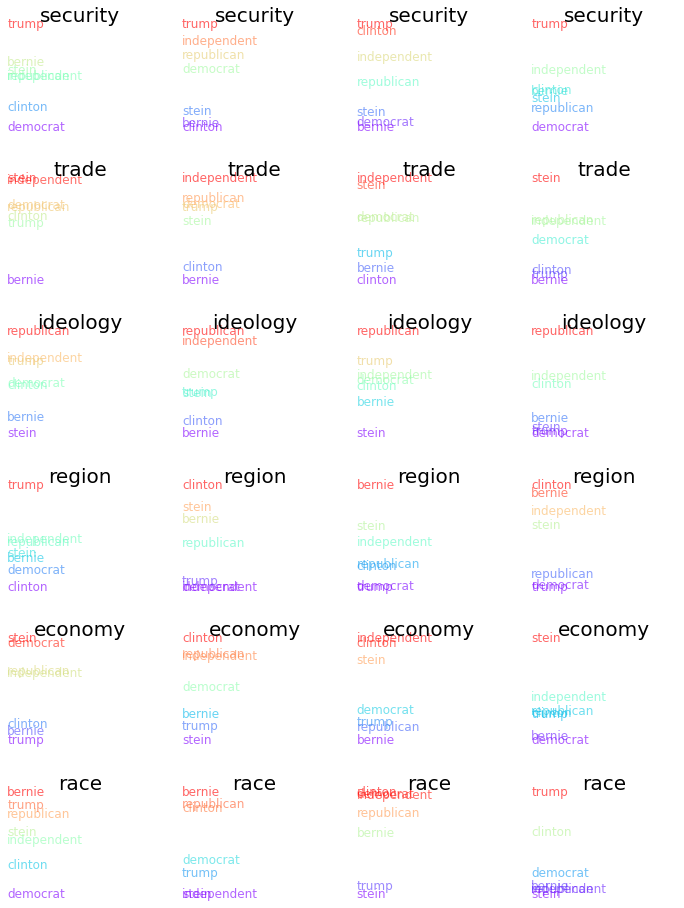
\includegraphics[width=0.95\textwidth]{figures/proj-candi.png}

    \caption{Projection of Candidate and Party names on dimensions of Security (strong-weak), Trade (local-global), Ideology (right-left), Region (urban-rural), Economy (rich-poor), and Race (american-immigrant). \\ From left to right, each projection refers to the time-window including (1) Super Tuesday in March 2016, (2) Elections in November 2016, (3) the first quarter of the presidency in Feb-Mar 2017, and (4) the `Unite the Right' rally in Charlottesville, August 2017}%

    \label{fig:proj_parties}%

\end{figure}
%--------------------------------------------------------%

\subsubsection*{Consistent perceptions of news outlets}

Figure \ref{fig:proj_media} provides a projection of news outlets -- print and Television -- on the aforementioned dimensions. I split them into these categories to disambiguate the different positions they take, and to examine equivalent pairs, like CNN-Fox, and NYT-Breitbart.

On the `Security' dimension in figure \ref{fig:proj_media}a, Fox News consistently ranks high relative, with MSNBC and CNN occupying the `weak' end of the dimension. The distance between Fox an the rest of the outlets from the second window onwards is indicative of the extreme posturing characteristic of their content. Fox also projects heavily on the `conservative' end of the ideology dimension, but it's surprising to see CNN show up there in the third window (first quarter of the Presidency).  

On matters of `Trade', MSNBC and CNN load heavily on the `global' end of the dimension. Other outlets like CBS and ABC promptly occupy the center on this dimension too. MSNBC and CNN occupy similar positions again on the `Economy' dimension, with the community perceiving them to be more closely associated with the `poor' end of the dimension. On questions of `Race' again, CNN stays reliably to the `immigrant' end of the dimension.

The consistency of the results persist with print news outlets too. National Review stakes its position as a conservative hawk on the Security dimension, its relative position far away from the other print outlets. The New York Times, Washington Post, and Wall Street Journal regularly load heavier on the `weak' end of this dimension, with Breitbart closer to the Review. The conservative nature of the Review persists on the Trade dimension, along with more globalist positions taken by the Times, Post and Journal.


% Projection of News outlets
\begin{figure}[t]%

    \centering

    \subfloat[Television News Media. Includes `MSNBC', `CNN', `ABC News', `CBS News', and `Fox News'.]{{ 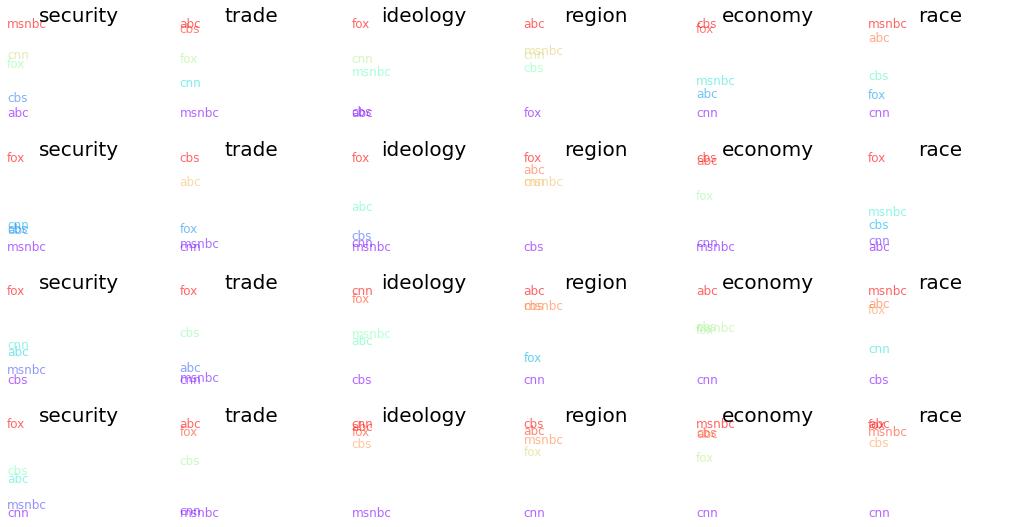
\includegraphics[height=0.38\textheight]{figures/proj-tv_news.png} }}
    
    \subfloat[Print News Media. Includes `New York Times', `Washington Post', `Wall Street Journal', `National Review', and `Breitbart'.]{{ 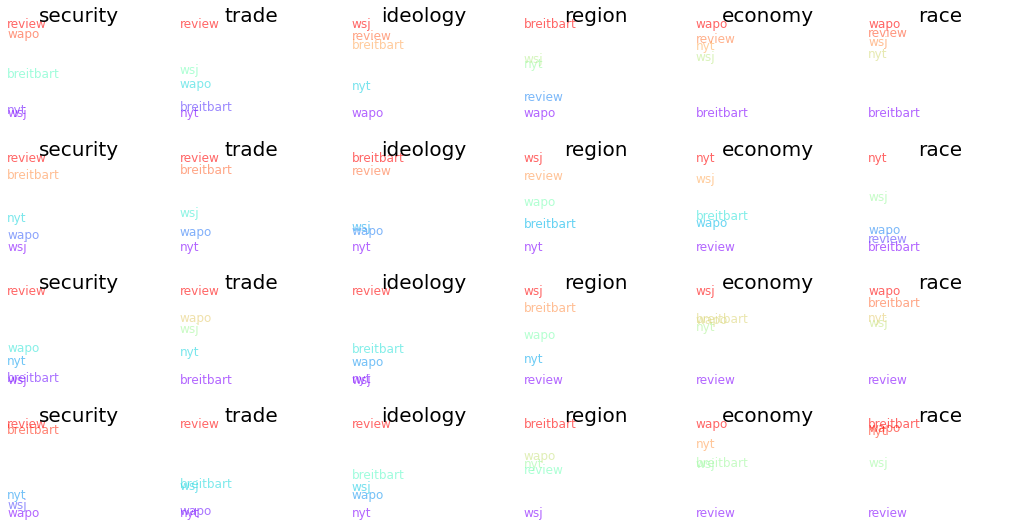
\includegraphics[height=0.38\textheight]{figures/proj-news.png} }}%

    \caption{Projection of Television and Print media outlets on dimensions of Security (strong-weak), Trade (local-global), Ideology (right-left), Region (urban-rural), Economy (rich-poor), and Race (american-immigrant). \\ From top to bottom, each projection refers to the time-window including (1) Super Tuesday in March 2016, (2) Elections in November 2016, (3) the first quarter of the presidency in Feb-Mar 2017, and (4) the `Unite the Right' rally in Charlottesville, August 2017}%

    \label{fig:proj_media}%

\end{figure}
%--------------------------------------------------------%









% \begin{equation}
% \label{eq:emc}
% e = mc^2
% \end{equation}



%------------------------------------------------

\section{Discussion}

The sharp increase in average cross-entropy for the community and top users in Period 10 is anomalous in several aspects. This period includes the weeks of the election, but it doesn't have the highest number of posts. But it does have the highest number of unique posters in our time-frame, a sharp increase from the previous period, even if the successive period, with its lower cross-entropy, doesn't see a sharp fall in posters (see Figure \ref{fig:sub_stats}).

Breitbart's position on the issue dimensions is an interesting case to examine. Given the consistency in the loadings of other outlets on these  dimensions, one would expect Breitbart to have a relatively stable position across these windows. Instead, what we see is that Breitbart's position shifts, closer at times to the conservative National Review and on the opposite end at others. One explanation for this could be that that constructed dimensions are not stable and don't encode the information we think it does. Testing and tuning these dimensions for greater reliability would be essential in making these results generalizable. An alternate hypothesis is that the nature of Breitbart's newsroom -- digital, highly partisan, more finely attuned to and reliant upon online communities for amplification -- make it fundamentally different from the more traditional outlets we compare against. Adding outlets like Vox Media, Huffington Post, or Buzzfeed could provide a third set of comparisons, among internet-first news outlets. But one could also examine how the language in Breitbart's articles linked on the subreddit align with the language in the subreddit. 

This paper examines how the linguisitic characteristics of a politically-engaged community changes with time, with an examination of how key phrases shift in accordance to events. We've been able to examine the relationship between a user's status and the language of the community, with our results replicating some of the findings in Danescu-Niculescu-Mizil et al.'s work. \citep{danescu-niculescu-mizil_no_2013}. Further work on this should focus on expanding beyond the $n$-gram model to quantify community language. Word Embedding methods which are able to better capture context could be used to identify more fine-tuned linguistic norms. Formalizing user status with centrality measures and sub-community network detection could help us tease out amplification channels within this community to examine in-group competition.      

%----------------------------------------------------------------------------------------
%	REFERENCE LIST
%----------------------------------------------------------------------------------------

% \begin{thebibliography}{99} % Bibliography - this is intentionally simple in this template

% \bibitem[Figueredo and Wolf, 2009]{Figueredo:2009dg}
% Figueredo, A.~J. and Wolf, P. S.~A. (2009).
% \newblock Assortative pairing and life history strategy - a cross-cultural
%   study.
% \newblock {\em Human Nature}, 20:317--330.
 
% \end{thebibliography}
\clearpage
\bibliography{bibliography.bib}

%----------------------------------------------------------------------------------------

\end{document}
